\documentclass[10pt,a4paper]{book}
\usepackage[utf8]{inputenc}
\usepackage{FiraMono}
\usepackage{lmodern}
\usepackage[T1]{fontenc}
\usepackage{xeCJK}
%\usepackage{CJKutf8}
\usepackage{amsmath}
\usepackage{amsfonts}
\usepackage{amssymb}
\usepackage{graphicx}
%\usepackage[cache=false]{minted}
\usepackage{tcolorbox}
\tcbuselibrary{minted}
\usepackage{chessboard}
\usepackage{hyperref}

%\usemintedstyle{colorful}

%\definecolor{bg}{HTML}{282828} % from https://github.com/kevinsawicki/monokai
%\definecolor{bg}{HTML}{BBBBBB} % from https://github.com/kevinsawicki/monokai
%\setminted{bgcolor=bg,breaklines=true}
%\setminted{breaklines=true,linenos=true,frame=single}
\begin{document}

\title{Data Structures}
\author{Andrew Rosen}
\date{}
\maketitle
\tableofcontents

%defs

\newtcblisting[auto counter,number within=chapter]{pycode}[2][]{%
	colback=black!5!white,
	colframe=blue!75!black,fonttitle=\bfseries,
	listing only,
	listing engine= minted,
	minted language=Python3,
	minted style=colorful,
	minted options={tabsize=4},
	title= Listing (Python) \thetcbcounter: #2,#1
}

\newtcblisting[use counter from=pycode]{javacode}[2][]{%
	colback=red!5!white,colframe=red!75!blue,fonttitle=\bfseries,
	listing only,
	listing engine= minted,
	minted language=Java,
	minted style=manni,
	minted options={tabsize=4,breaklines=true},
	title= Listing (Java) \thetcbcounter: #2,#1
}

%\newtcblisting[use counter from=pycode]{pyfile}[2][]{%
%	colback=black!5!white,
%	colframe=blue!75!black,fonttitle=\bfseries,
%	listing only,
%	listing engine= minted,
%    listing file=#2,
%	minted language=Python3,
%	minted style=colorful,
%	minted options={tabsize=4},
%	title= Listing (Python) \thetcbcounter: #2,#1
%}

\newtcblisting[use counter from=pycode]{pyfile}[2][]{%
	colback=black!5!white,
	colframe=blue!75!black,
	fonttitle=\bfseries,
	listing only,
	listing engine=minted,
	listing file=#2, % Correct key for specifying the file with minted
	minted language=Python3,
	minted style=colorful,
	minted options={tabsize=4},
	title=Listing (Python) \thetcbcounter: \ifx\\#1\\#2\else#1\fi % Use #1 as custom title or fallback to filename (#2)
}


%The Document 
\part{Preliminaries}

\chapter{Introduction}

\section{What is a Data Structures Course}
Data Structures is all about defining the different ways we can organize data.  This is not databases, which is concerned with defining the various attributes of a bunch of data;  this is much more granular.  We want to know how to store and retrieve a single item of data.


\section{Why This Book?}

This textbook is free.

It is both Java and Python, which is a bit insane.  You have two valid choices: 
\begin{itemize}
	\item 
	\item Understand that the concepts we are learning are way more important than the language and treat the other language as psuedocode (which isn't hard for Python)
	
\end{itemize}
be comfortable in multiple languages and embrace being a polyglot


\subsection{Where Does This Book Fit Into a Computer Science Curriculum }

Education in Computer Science is based around three core topics: translating the steps of solving a problem into a language a computer can understand, organizing data for solving problems, and techniques that can be used to solve problems. % reword
These courses typically covered in a university's introductory course, data structures course, and algorithms course respectively, although different universities decide exactly what content fits in which course.
Of course, there is are lot more concepts in computer science, from operating systems and low level programming,  to networks and how computers talk to each other. However, all these concepts rely on the knowledge gained in the core courses of programming, data structures, and algorithms.



This textbook is all about Data Structures, the middle section between learning how to program and the more advanced problem solving concepts we learn in Computer Science. 
Here, we focus on mastering the different ways to organize data, recognize the internal and performative differences between each structure, and learn to recognize the best (if there is one) for a given situation.


\subsection{What Are My Base Assumptions about the Reader?}

This textbook assumes that the student has taken a programming course that has covered the basics.
Namely: data types such as ints, doubles, booleans, and strings; if statements, for and while loops; and object orient programming.
This book is also suitable for the self taught programmer who has not learned much theoretical programming

\section{To The Instructor}

You'll note that this textbook lacks some of the features found in commercially available textbooks.  The biggest of these is slides.  



For the most part, slides are too static to help students understand how to code. 



Does the lack of varied exercises make cheating on assignments easier as semesters go on?  Yes, but that bridge was burned long ago.  
The cheating student can plagiarize from various websites or anonymously hire another to do their work for them.
However, the student who cheats isn't exactly clever and certainly hasn't been exposed to much game theory.  
They will often cheat from the same source.  

In addition, during the writing of this text, technologies such as GPTChat were released.  This hasn't so much burned the bridge as dropped napalm on the entire surrounding forest.  Newer technologies will then salt that earth. I recommend an open and honest dialogue with your students and at least 50\% of their grade being the result of evaluations and assessments you do in class.  This can range from proctored exams to flipping the classroom and giving students the chance to work  on homework in class, where they are much more likely to turn to you or their peers for help.


\subsection{Assignments}
I will drop the sporadic assignment here or there, drawing from the same places you should draw from:
\begin{itemize}
	\item Nifty Assignments
	\item  Problem Solving with Algorithms and Data Structures using Java (Miller)
\end{itemize}

\subsection{How to Use}

%TODO create tag for teacher edition
\section{To The Student}



Why are we learning this?  As Brad Miller and David Ranum put in their aforementioned book (which is creative commons and you should totally check out):

\begin{quotation}
	
	To manage the complexity of problems and the problem-solving process, computer scientists use abstractions to allow them to focus on the “big picture” without getting lost in the details. By creating models of the problem domain, we are able to utilize a better and more efficient problem-solving process. These models allow us to describe the data that our algorithms will manipulate in a much more consistent way with respect to the problem itself.
	
	Earlier, we referred to procedural abstraction as a process that hides the details of a particular function to allow the user or client to view it at a very high level. We now turn our attention to a similar idea, that of data abstraction. An abstract data type, sometimes abbreviated ADT, is a logical description of how we view the data and the operations that are allowed without regard to how they will be implemented. This means that we are concerned only with what the data is representing and not with how it will eventually be constructed. By providing this level of abstraction, we are creating an encapsulation around the data. The idea is that by encapsulating the details of the implementation, we are hiding them from the user’s view. This is called information hiding.
	
	Figure 2 shows a picture of what an abstract data type is and how it operates. The user interacts with the interface, using the operations that have been specified by the abstract data type. The abstract data type is the shell that the user interacts with. The implementation is hidden one level deeper. The user is not concerned with the details of the implementation.

	
	Figure 2: Abstract Data Type
	
	The implementation of an abstract data type, often referred to as a data structure, will require that we provide a physical view of the data using some collection of programming constructs and primitive data types. As we discussed earlier, the separation of these two perspectives will allow us to define the complex data models for our problems without giving any indication as to the details of how the model will actually be built. This provides an implementation-independent view of the data. Since there will usually be many different ways to implement an abstract data type, this implementation independence allows the programmer to switch the details of the implementation without changing the way the user of the data interacts with it. The user can remain focused on the problem-solving process.

\end{quotation}

\subsection{How to use}



%\section{Science and Art}

% license  and ack https://runestone.academy/ns/books/published/pythonds3/index.html?mode=browsing after adapting text.
\chapter{Functions and How They Work}

This will be an extremely short chapter, but an important one.

\section{The Runtime Stack}


\section{Passing Arguments}

\subsection{How it Works in Java}

\subsection{How it works in Python}


\chapter{The Array}

\section{Why Arrays}

\begin{itemize}
	\item because new language: 
	Since this is a data structures course, I assumed that students have had exposure to arrays or array like objects.
	This chapter goes into a bit of a deeper detail that may have been glossed over and Introduces the topic in the appropriate language if need be.
	
	In other words, I assume you know what an array is , but not necessarily how to use it in Java or Python\footnote{Although we use lists in python}.
	\item  because internal memory lookup
	\item Because we need to make sure internal knowledge is cohesive (eg arrays of objects are arrays of pointers/references)
\end{itemize}







\section{Java and Arrays}
The Array is a built in class in Java, but the syntax is a bit unique \footnote{Enough so that I constantly had to look up how to do it my first two years of undergraduate studies, so don't feel too bad if you have to do the same.}

To create an array in Java we do:

\begin{minted}{Java}
	Type[] myArray = new Type[sizeOfArray]
\end{minted}


Here, every item in the array is of whatever \texttt{Type} we want, which could be a Class or primitive.   
Arrays can be whatever integer size we desire, but once set it cannot be changed.
This is because to create an array, the computer allocates a contiguous block of memory.
If we wanted to resize it, there is no guarantee that this chunk of memory won't have things directly before or after it, preventing us from safely extending its range.

\section{Python and Arrays}
\label{sec-python-arrays-lists}
Python doesn't really do arrays in the same way.
It instead uses Lists, as we'll see in Chapter \ref{chap-arraylist}.
\texttt{myNotArray = []}\footnote{On styles:  Java convention is to use camel case for variable types (\texttt{myVariableName}), while python convention is to use underscores (\texttt{my\_variable\_name}).  I will be using the Java style camel-casing for variables throughout the book for consistency and because it is my preference.}  does not actually make an array like you assume it would in some other language.  Instead it makes A list (specifically an array list ) to contain these items.
This works exactly like an array in other languages, but you get access to some nifty operations in Python, like slicing, concatination, and  builtu in methods.  In addition, Python dynamically resizes this array if we need it bigger or smaller.\footnote{We cover the specifics in Chapter \ref{arraylist}}



However, if you really want or need to use an array in python, you can.
%TODO factcheck
There are two ways to accomplish this.
The first way is the built in \texttt{array} package.  This builds a wrapper for the more primitive but efficient c-based array. 
The python package \texttt{numpy} contains yet \textit{another} type of array, this time much more focused on mathematical operations. 
In short, if you're working in python, use a list unless you know you should use something more specialized.







\section{How an Array Works}

As previously mentioned, an array creates a contiguous block of memory.  But what does this actually mean?
%autogenerated placeholder diagram  by chatgpt
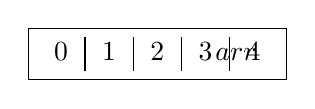
\begin{tikzpicture}
	\node[rectangle, draw] (array) {
		\begin{tabular}{c|c|c|c|c}
			0 & 1 & 2 & 3 & 4 \\
		\end{tabular}
	};
	\node[right of=array] (label) {$arr$};
\end{tikzpicture}

Here, $arr$ does not contain the array; it hold the memory location, the reference, the pointer to the array.  The correct term varies on the language you are using, but the point is that $arr$ tells you the location of the array rather than holding the array itself.


\subsection{Operations}

To review, arrays have two operations and one attribute: storing  a value at an index, retrieving a value from an index, and obtaining the size. 


For an array $arr$, retrieving a value from an array is and storing it in some variable is done with:

\begin{verbatim}
	myVar =  arr[index]
\end{verbatim}

and to store something in $arr$, you use:

\begin{verbatim}
	myVar =  arr[index]
\end{verbatim}


Interestingly enough, this is one of the few consitant accross multiple programming languages.

Figuring out the length of an array in Java\footnote{This is one of the little things in Java that can be a source of frustration.  Strings use \texttt{.length()}, arrays use \texttt{.length}, and Collections like Lists and Sets use \texttt{.size()}.} is done with 

\begin{minted}{Java}
	int len =  arr.length;
\end{minted}

and in python, a simple \texttt{len(arr)} works.

\subsection{Array Internals and the Memory Formula}
So how does an array actually work?  How do you actually retrieve a value from an index?
The most crucial thing to keep in mind in this textbook is when you see something like the code below:
\begin{verbatim}
	variable = expression;
\end{verbatim}

The left side is always a variable.  The expression on the right side always\footnote{except for primitives, like \texttt{int} in Java} yields some memory location.  This means you should repeat to yourself ``the memory location on the right gets stored in the variable on the left.''

This means that 
\begin{minted}{Java}
	int[] numbers = new int[10];
\end{minted}

stores a memory location in \texttt{numbers}.  It does not store 10 integers in \texttt{numbers}.  It only tells you where to find them.  Specifically, it stores the memory location of index 0 of the array.  This is true for not only Java, but C as well, and almost every programming language\footnote{Python and other interpreted languages are slightly more complicated because we are dealing with array lists, thus one additional level of abstraction, so this storage just happens a layer deeper.  Esoteric languages like ook prevent me from making a statement like ``all languages.'' }. 


This means that 

What if we aren't dealing with primitives, but with objects like Strings instead?





\section{Common Array Algorithms}

\subsection{Finding Values in an Array}
\subsubsection{Finding the Minimum}

\subsubsection{Finding the Average}


\subsection{Limitations}
Arrays are awesome solutions for many problems, but they are lacking in ability for some problems.  Consider the following exercise:

\begin{verbatim}
	
	Given a string of text, determine what the most common character of text is. 
	
\end{verbatim}
Unless you've seen this problem before, there is no obvious solution.  Considerable thought eventually lands on an idea: characters are just integers, so we could assign each one of the characters an index and increment the index each time we see the character.

\begin{minted}{Java}
public static char mostFrequent(String text) {
	int[] tally = new int[128]; 
	for(char c : text.toCharArray()) {
		tally[(int) c] += 1;
	}
	
	indexWithHighest = 0;
	for(int index = 0; index<128; index++) {
		if( tally[index] > tally[indexWithHighest]){
			indexWithHighest = index;
		}
	}
	return (char) indexWithHighest;
}

\end{minted}

\begin{CJK}{UTF8}{min}However, this has some serious limitations.  For one, this breaks if we are not using ascii.  What if the text is ``こんにちは'' or other non-english text?
\end{CJK}
You could create a larger array for all 100000+ unicode characters, but this begins to become less and less feasible.  
And now what if we change the problem to:

\begin{verbatim}
	
	Given a string of text, determine what the most common word is. 
	
\end{verbatim}

This suddenly becomes an extremely annoying problem to solve with just arrays\footnote{Those of you coming from Python can stop shouting ``use dictionaries!'' at the top of your lungs.}.  We will solve this problem when we visit Maps in Chapter \ref{chap-maps}, which are much better suited for this job than arrays.

The other limitation of arrays  that their size is immutable.  Once an array has been declared, we cannot change its size.  This is rather inconvenient for a number of applications where we may not know how many items to store.  This will be the focus of our first new data structure:  The List.



\chapter{Analyzing Algorithms}
Or we would look at the list, but we need to talk about Math.  Sorry for the bait-and-switch, but it will make sense shortly.


You don't need  much math to be a good programmer, but if you want to be an amazing programmer, you probably need math or very math adjacent skills.
\section{Cost}
Every function, operation, algorithm, or what have you that a computer performs has a \emph{cost}. 
In fact, there are always multiples costs;  we often just focus on the most important one or two costs.  

What is most important depends on context.
However, in the vast majority of cases, the most important cost to focus on is \textbf{time}.
When our program is eating away at our storage resources like a hungry child slurping up spaghetti, we can always go out and buy more memory/storage/RAM.
If our program requires a large amount of energy consumption, energy is readily available from a variety of sources: batteries, power plugs, internal combustion engines, the giant fusion reactor in the sky.




\subsubsection*{Measuring Cost}
When we measure cost, we need to do abstractly.  
When we measure the amount of time that an algorithm takes, we look at the number of operations that will be executed, not the overall elapsed time.

\subsection{Time}
A time cost is a measure of not just how long it takes a program to finish executing, bit also how the length of execution is affected by adding additional item.

Time is almost always \emph{the most important cost}. We cannot got out and buy another weeks worth of time.  You can't hand a bunch of money to the reaper and ask for a deferral. You can't buy another minute to spend with your mother\footnote{Call your mother.  She would love to hear from you.} 
Yes, processors get faster as technology marches on, but they get faster slowly and Moore's law ostensibly has its limits.
The only way to make our programs realistically run faster is to make them more efficient.  And \textbf{Big O notation} is the way we will be measuring that efficiency.


\subsection{Space}

For data structures, we will be measuring their space efficiency in terms of \textit{auxiliary} cost, in other words, how much extra space we need to use over the space used for the items itself.   To clarify, any data structure that contains $ n $ items of roughly the same size will use $ n \times \mathtt{sizeOf(item)}$ space at minimum, no matter what data structure we use.  This accounts for the 
Each data structures 

\subsection{Energy}
%\subsection{Other costs - Bandwidth}
While not something this book concerns itself with, some programmers need to be wary of the amount of energy  an algorithm consumes.  If energy is expensive and/or battery life needs to be conserved, then choosing an energy efficient algorithm might be a better choice, even if the time or space complexity is higher.  Some examples where energy use is a large concern  is Mobile Ad-Hoc Networks (MANETs) and battery powered cameras.


\section{Big O Notation}

\begin{itemize}
	\item What is big O
	
	\item  how to read it
	\item Aside about big omega and theta
	\item How wrong usage annoys mathematician
	\item refers to cost in general, but used for time usually
	\item  space complexity 
	\item Common runtimes
	\item runtimes we''ll focus on now
	\item runtimes we focus on later
\end{itemize}



\subsection{Space Complexity}

\section{Examples with Arrays}

\begin{itemize}
	
	\item Retrieval  - refer back to earlier chapter for address lookup 
	\item Replacement
	\item Linear Search
	\item Binary Search
\end{itemize}



\subsection{Selection Sort}



\subsection{Bubble Sort}
\subsection{Insertion Sort}
\subsection{Other Sorting Algorithms}


\section{The Formal Mathematics of Big O Notation}
\section{Other Notations}


\section{When To Ignore Costs}

\part{Lists}
\label{part-list}


\chapter{Array Lists}
\label{chap-arraylist}
%TODO Find the Ur List and Ur dynamic array
The first data structure we will be studying is the list.
The list is by far the most relatable data structure, as humans deal with lists on a regular basis.

\section{What is a List?}


When you get right down to it, lists are defined by order.
We don't have to take advantage of this order, but its there.
Populated lists have a first item and they have a last item.

Take a look at this quest below from a hypothetical fantasy game:

\subsubsection*{Quest: Slay the Dragon of Doom}
\begin{itemize}
	\item Get Sword of Dragonslaying
	\item Locate the map to Dragon Lair of Doom
	\item Travel to the Dragon Lair of Doom 
	\item Slay the Dragon of Doom
	\item Return to the Castle
\end{itemize}

Here, the order is implied by the contents of the list - you can't beat the dragon without the macguffin and you certainly can't fight it without being able to find it.
Generally speaking, going up against a dragon without any preparation is foolhardy in the extreme, but I digress.

Thus, you must get the special sword\footnote{What if its possible to get the map before the sword? We'll see much later this kind of quest and it's requirements are much better handled by a directed acyclic graph in Chapter \ref{chap-graphs}, but this example is fine for teaching lists.} first, and you must get the map to find the lair before you can physically travel there.

\subsection*{shopping list example}
While lists are defined by order, we don't necessarily  need to ascribe any meaning to the order.
Take a look at the shopping list below:




<Shopping List>
While bread is the first item on this list, being the first item in the shopping list in this case has no special meaning.  It's not the most important item on the list\footnote{obviously, that's the cookies}, nor is it necessarily the item I'm going to pick up first.

Where arrays and lists differ is that lists can grow to an arbitrary size, whereas

\begin{itemize}
	\item Lists can grow to any arbitrary size, but lists  
\end{itemize}

Data in a list is stored sequentially and array lists do this by creating a an 


\subsection{A note on terminology}
An \textbf{array list} is a type of list.  These are sometimes called dynamic arrays.

As mentioned in Section \ref{sec-python-arrays-lists}, Python doesn't have arrays.  If you've been programming in Python, you've been using an array list the entire time you've declared \texttt{[]}.  They are usually just called lists rather than array lists.


I will be using the Java nomenclature for the majority of the book as this allows me to be clear about the types and implementations of data structures.

\subsection{Lists in Java}

So what does

\subsubsection{An Aside about interfaces}
\subsubsection*{Here is the source code}



\section{Generics}

\subsection{What are they?}


Before we get to deep into lists, we need to have a discussion about generics. Generics are a way of restricting and specifying what types can go into a collection.

\subsection{But Why?}




\section{List Operations}


\subsection{Size} We need some easy way of knowing how big our lists are, if for no other reason than to make sure our  add and remove methods can figure our their valid indices.


\subsection{Add}  By default, we add items to the end of the list, but we can also add items to any index we want.

When we add an item at some specific index $ i $, the item at $ i $ and all indices to the right shift over one.  In other words, what was at $ i $ is now at $ i+1 $, what was at $ i+1 $ is at $ i+2 $,  and so on.

This also an understandable restriction to adding items to a list -  we cannot an item to any index greater than \texttt{myList.size() +1}.   Anything greater wouldn't be at the end of the list; it would be beyond it.  The same goes for negative indices.
 
<possible picture showing a legal an illegal add>

%We will cover this operation in more detail when we implement the add method for the arraylist 

\subsection{Remove}  We can remove Items from a list much in the same way we can add them. When removing an item at index I , all the indices to the right shift one over to the left 
\subsection{Get}
\subsection{Set}

\section{ArrayLists}
An array list, as you might have guessed, are lists built using \textit{arrays}.\footnote{Shockingly, many of the names we give things at this point actually make sense.}
They work by growing or shrinking the array\footnote{A lie.  As you'll see we don't actually change the size of an array;  we create a new array of the appropriate size and copy everything over} automatically as items are added or removed from the list, giving the illusion that the data structure can hold an arbitrary amount of data.

We'll go into the specifics of how this works in Section \ref{buildingArraylist}.


\subsubsection{Java's ArrayLists}
Java's arrayList
\subsubsection{Python's Lists}
Python's lists, such as below:
\begin{minted}{python3}
	l = [1,2,3] # this is a list, not an array!	
\end{minted}
are actually array lists! %TODO cite this https://docs.python.org/3/faq/design.html#how-are-lists-implemented-in-cpython

Python uses a different vocabulary for some of the methods we'll be implementing below.  
For example, take the action of adding an item to a list.
Python uses the \texttt{append} method to add an item to end of the list and \texttt{insert} to put an item into the middle of the list.
Java (who's vocabulary we'll be following), uses \texttt{add} for both these contexts. 









\section{Example Algorithms}


\begin{minted}{Java}
	public static <E> boolean isPermutation(List<E> listA, List<E> listB) {
		
		if(listA.size() != listB.size()) {
			return false;
		}
		for(int i  = 0; i < listA.size() ; i++){
			E item =  listA.get(i);
			int countA = 0;
			int countB = 0;
			
			for (E element : listA) {
				if(item.equals(element)){
					countA++;
				}
			}
			for (E element : listB) {
				if(item.equals(element)){
					countB++;
				}
			}
			if(countA != countB) {
				return false;
			}
		}
		return true;
	}
\end{minted}



\section{Building an ArrayList}
\label{buildingArraylist}
To truly understand how a data structure works we need to implement it ourselves.

\subsection{Caveats}

\subsubsection{MyArrayList.java}
We will not be implementing the \texttt{List} interface. We don't need to implement all the functions to get an understanding of how the fundamentals of an arraylist work.
Implementing the list interface would take up a hideous amount of physical space and get in the way of actually understanding the code.



\subsubsection{myArrayList.py}

For python, this will require some suspension of disbelief, as our array list will require using an array, and as previously discussed, arrays are shirked in favor of arraylists in python.  We'll be using a list and pretending it's an array. Silly?  Yes.  But it will keep our code compact and easier to understand.

%Remember, the standard python list is built in the C programming language.

\subsection{Instance Variables}

Believe it or not, we only need to keep track of three instance variables to get our arraylist working.

\begin{enumerate}
	\item[theData]  We need an array to actually store the items.  This is it.
	\item[size] Size here refers to the total number of items we have stored in the array.
	\item[capacity]  This is the number of items  the underlying \texttt{array} in our list can hold. It is the maximum size of the list before we have to do something about it. This is not strictly necessary as we can get it by querying \texttt{array}'s length. However, making it it's own variable will help with the readability.
\end{enumerate}

It is very easy to confuse size and capacity since they both deal with counting how many elements.  When I talk about \texttt{size}, I am talking about the number of items we have stored in the list we are making.  Capacity, on the other hand, depends on the length of the built-in array. 

\subsubsection{Java}


\begin{minted}{Java}
public class MyArrayList<E> {
	
	private E[] theData
	private int size;  // how many items are in the list
	private int capacity;  // how many items the underlying array can hold
	
	
\end{minted}

First, note the \texttt{<E>} after \texttt{MyArrayList}.  This means that we're saying:
\begin{itemize}
	\item MyArrayList is designed to hold a specific type of object.
	\item Every \texttt{E} we see is a placeholder for some type, which will be that same across the entire lifespan of the object.
\end{itemize}


\subsubsection{Python}
\begin{minted}{Python3}
class MyArrayList(object):
	pass
\end{minted}


\subsection{Constructor}

We need to set the variables to their initial values upon creating the arraylist.
The \texttt{size} will be 0, since we won't have any objects stored in it yet.
We will set the \texttt{initial} capacity to 10.  
It's a small number and thus won't create much wasted space if we don't fill up \texttt{theData}.
\texttt{theData} will be an empty array of \texttt{capacity} length.
If \texttt{theData} becomes full, we will create a bigger array to hold our items using the \texttt{reallocate()} method (Section \ref{
arraylist-reallocate})  %TODO Subection Depth


\subsubsection{Java}
With our constructor, we have one line of weird black magic in order to create an Array of \texttt{E[]}'s.
\begin{minted}{Java}
public MyArrayList(){
	size = 0;
	capacity = 10;
	theData = (E[]) new Object[10]; // this generates a warning
}
\end{minted}

So what's going on with the last line?
Typically, when creating an array, we would just say:

\begin{minted}{Java}
//doing this in the constructor gives us an error.
TYPE[] myArray  = new Type[desired_size];
\end{minted}

However, Java won't let you create new \texttt{E} objects since there's no telling what the constructors will be.  This rule extends to arrays of \texttt{E}, like so:
\begin{minted}{Java}
theData =  new E[10];
\end{minted}

However, when creating a new empty array of objects of any type, we're just making an array of nulls which will eventually be replaced by references to objects.  Thus, even though the Java compiler will yell at us about Type safety, we can instead create an array of \texttt{Object} and then tell , since all references to any types are the same size.

\begin{minted}{Java}
// creating one array of nulls and telling Java 
// its another type of array of nulls. 
theData = (E[]) new Object[10];
\end{minted}



Remember how Java and most modern programming languages deal with objects; if you're assigning an object to a variable, like in \texttt{Object o = new Object()}, we are storing a reference to that object.

Thus, when we add an item to a list, what really happens is we'll be adding a reference to it - the instructions on how to find it in memory.
\subsubsection{Python}
Python is fairly straightforward, with the caveat that we are pretending \texttt{theData} is an array, and not a list.

\begin{minted}{Python3}
class MyArrayList(object):
	def __init__(self):
		self.size = 0
		self.capacity = 10
		self.theData = [None]*self.capacity
\end{minted}

Since built-in lists in Python grow and shrink like we would expect a list to, we initialize \texttt{theData} with 10 \texttt{None} objects\footnote{This is the Python equivalent to the Java \texttt{null}.} to mimic the way an array would be initialized.


%\subsection{Placeholder toString}
%
%
%\subsubsection{Java}
%
%\subsubsection{Python}

\subsection{Size}
Now, we will add a size method to our list; fairly straightforward in \texttt{Java}.

\begin{minted}{Java}
public int size() {  
	return size;
}
\end{minted}

In Python, we can go ahead and use the built in \texttt{\_\_len\_\_} method.

\begin{minted}{Python3}
def __len__(self):
	return self.size
\end{minted}

Which can then be invoked with \texttt{len(myList)}.


It is worth reinforcing that by keeping track of the size in a variable, retrieving the size of our list is always $O(1)$

\subsection{Add}



In Python, these two \texttt{add} methods are called \texttt{append} and \texttt{insert} respectively, as python does not support method overloading.

\begin{minted}{Java}
public void add(int index, E item) {
	if(index < 0 || index > size) {
		throw new IndexOutOfBoundsException("Index " + index + " out of bounds.");
	}
	
	if(size == capacity) {  // O(n) time...sometimes.  Amortized over the cost of adding
		this.reallocate();
	}
	
	for(int i = size - 1; i >= index; i--) { //If adding to the end... constant
		E temp = theData[i];
		theData[i+1] = temp;
	}
	
	theData[index] = item;
	size++;
}
\end{minted}


\begin{minted}{Python3}
def insert(self, index, item):
	
	
	self.size += 1

\end{minted}





Finally, since adding to the end is an extremely common operation, we will overload our \texttt{add} method.
If our list is provided with only an \texttt{item}, as opposed to an \texttt{item} and an \texttt{index}, we will just add that \texttt{item} to the end.
Since we already wrote a perfectly good \texttt{add} method already that we know works, we'll just have our new method call that one.
\begin{minted}{Java}
public boolean add(E item) {
	this.add(size, item); // size is the last valid index
	return true; // What?
}
\end{minted}

Why are we returning \texttt{true} here?
The short answer is practice and consistency with future data structures.
The long answer is any \texttt{Collection} in Java has must have an \texttt{add} method and a \texttt{List} is type of \texttt{Collection}\footnote{Our \texttt{MyArrayList} isn't technically a \texttt{Collection} since we did not implement the \texttt{List} interface, but I digress.}.

\texttt{Collection} specifies that \texttt{add} must take in an \texttt{item} and return a \texttt{boolean}.
A \texttt{true} signals the \texttt{add} is successful.
A \texttt{false} signals that we could not add the \texttt{item}.
For example, this might happen with a \texttt{Set} (Chapter \ref{chap-sets})


On the other hand, our Adding at a specific index is unique to lists, and not part of collections,  and will always work. Therefore, there's no need to return a boolean. 

\subsubsection{Reallocation}
\label{arraylist-reallocate}
When we need to grow our arraylist
%TODO fix this code or ensure that capacity is doubled before copying
\begin{minted}{Java}


private void reallocate(){
	//doubles or 1.5x capacity
	//don't do +1 capacity
	E[] newData = (E[]) new Object[capacity];
	for(int i = 0; i < theData.length; i++) {
		newData[i] =  theData[i];
	}
	
	theData = newData;
	capacity = 2 * capacity;
	
}
\end{minted}

We want to double our capacity or at least increase it by 50\%, Rather than increasing it by a static number.
Consider if we increase the capacity by one each time we reallocated.  If we did that, we would have to reallocate every time we added a new item to the list.  This would mean that every time we add an item to list, add becomes a linear time - $O(n)$ - operation.

%TODO explain what happens to runtime amortization when we reallocate but double the size

\subsection{toString and \_str\_}
Now that we supposedly have a method for adding items into the list.


\subsection{Get and Set}
The \texttt{get} and \texttt{set} methods are fairly straightforward:
\begin{enumerate}
\item[\texttt{get} -] Given an \texttt{index}, retrieve the item stored at that \texttt{index}.
\item[\texttt{set} -] Given an \texttt{index}, replace the old item stored at that \texttt{index} with the provided \texttt{item}.
\end{enumerate}
%For \texttt{get}, given an \texttt{index}, retrieve the item stored at that \texttt{index}.
%For \texttt{set}, given an \texttt{index}, replace the old item stored at that \texttt{index} with the provided \texttt{item}.
\texttt{set} has one additional quirk, we also want to return the old item we're replacing, just in case the programmer wants to doing something with the old item.
This would obviate the need for pairing a \texttt{get} and \texttt{set} call with each other if we want to replace the old item, but do something else with it. 

For both \texttt{get} and \texttt{set}, we want to throw some kind of error if the provided index is out of bounds.
\subsubsection{Java}
Our \texttt{get} is fairly straightforward, but feel free to give more information with the error.
\begin{minted}{Java}
public E get(int index) {
	if(index  < 0 || index >= size) {
		throw new IndexOutOfBoundsException("Index " + index + " out of bounds.");
	}
	return theData[index];
}
\end{minted}

The same goes for our \texttt{set} method. 
\begin{minted}{Java}
public E set(int index, E item) {
	if(index < 0 || index >= size) {
		throw new IndexOutOfBoundsException("Index " + index + " out of bounds.");
	}
	E oldItem  = theData[index];
	theData[index] = item;
	
	return oldItem;
}
\end{minted}

\subsubsection{Python}

Python supports negative indices.  It's up to you whether or not you want to support that, but if you do you need to account for the \texttt{capacity} and the \texttt{size} of the internal list.


We can take advantage of some of the method calls built into python to make our \texttt{myarraylist} support indexing.


\subsection{Remove}




\section{Analysis}

\section{More Restrictive or Permissive Generics}

\section{A Few More Useful Methods}

\subsection{Constructors}
Java's \texttt{ArrayList} can optionally take in an integer as an argument

\subsection{Trim}

The \texttt{trim()} exists to mitigate the fact that arraylist capacity and size don't often match up.


On the other hand, Python will automatically optimize lists for you CITATION NEEDED.

For other languages, check to see if the equivalent exists

\subsection{Adding Multiple Items in One Invocation}
One common operation is to move or copy all the items from one list to another.
In Java, we can use the \texttt{addAll()} method, which takes any Java collection as a parameter and all the items in that collection to the object.

\begin{minted}{Java}
List<Integer> a =  new ArrayList<>();
List<Integer> b =  new ArrayList<>();
for(int i = 0; i <3; i++) { 
	a.add(i); 
}
for(int i = 3; i <6; i++) { 
	b.add(i); 
}
a.addAll(b);
System.out.println(a); // 0 to 5 inclusive
System.out.println(b); // [3, 4, 5]
\end{minted}

In Python, we can use the \texttt{extend()} method on anything that is iterable or use some clever slicing.  However, I would always recommend using the method call over the slice, since a method invocation is always more readable.


\begin{minted}{Python3}
a = [0, 1, 2]
b = [3, 4, 5]
c = a + b # creates a new list, which is not extend
a.extend(b) # adds all of b's items to a
a[len(a):] = b # does the same thing but unreadble.
\end{minted}
A common beginner mistake in Python is to try to extend a list by calling \texttt{append} on the list like so.

\begin{minted}{Python3}
a = [0, 1, 2]
b = [3, 4, 5]
a.append(b) # a is now [0, 1, 2, [3, 4, 5]]
\end{minted}



This adds the entire list a single item in the list.  

\chapter{Linked Lists}
Linked lists , also referred to as reference based lists , are the second type of lists typically seen in applications . To be clear a linked list is a list. That means it could be used anywhere an array list can.   So Why do we have two objects that are functionally equivalent , two collections that hold things in order, using indexes?  The answer is will see, is because each list is good at the thing the other list is less efficient at.


Array based lists use contiguous blocks of memory, allocated all at once and when then capacity of the list is filled up.  Utilizing an array makes these types of lists extremely efficient at retrieving an item from a specific index, but adding items anywhere but the end of the list incurs a $O(n)$ runtime.



Linked Lists can do all the things an Array List can, but the underlying structure is completely different.  
Each item in the list is stored in an Object called a \textit{Node}.  Nodes are created as items are added to list, rather than in advance.  This means that are not contiguous, but Rather they are scattered throughout the computer's memory . So how in the world do we keep track of where we've stored all these items ? The solution resembles the scavenger hunt through the computer's memory.  Each node Not only the memory location of the item that is being stored, but the memory location of the next node in the list . An example of this code can be found below\footnote{Why is this class private in Java \texttt{private}? An inner class  (or private class) is a class that lives within another class.  We use this for two reasons:  Our nodes only exist to build the linked list, so they don't need to have their own class.  The Second reason is   What about \texttt{static class}? This means that we can create nodes without having to make a Linked List first! }: %TODO Check this.

\begin{minted}{Java}
	// a snippet of the Node Class
	// This will live inside the LinkedList class
	private static class Node<E> {
		E item;
		Node<E> next;
		
		public Node(E item) {
			this.item =  item;
		}
	} 
\end{minted}
Upon first glance, this code may be very confusing. Each node class contains a reference to a node inside of it.  This may give the impression that nodes  situated one inside another, like one of those Russian nesting matryoshka dolls.  
However, keep in mind what the node is actually storing is not other objects, but instead memory locations of where to find them.
This means that our linked list is more akin to a scavenger hunt where each objective in the hunt contains the instructions on how to find the next objective.

In other words, the item Is the data that is being stored (well actually the memory location, don't forget that ) , and next refers to the memory location of the next index in the list.  Crash course is an excellent video demonstrating this which you can find here: %TODO: Link video


\section{Connecting Nodes into a list.}
%TODO





we keep track of only the first and last item in the list, referred to as the head and the tail . 


I will be presenting the directions to building a fully functional  singly-linked list and doubly-linked list.  
These directions will differ from the mechanics of how your programming language of choice implements them, but have the same time complexity for their operations.
My implementation is constructed with the goal of making the code easy to understand and the decisions that need to be for adding and removing reflect each other.
Finally, my code aims to minimize the number of null-pointer exceptions and their ilk a programmer would make.

The full implementations can be found at the end of the Chapter.

\section{Building a Singly LinkedList}
We open up our linked list with a class declaration. 
If our language uses generics, we specify it there.
I'll be choosing not to inherit from the built-in list so we can focus solely on our own code and no external distractions.


In Java, our code begins like this.
\begin{minted}{Java}
	public class LinkedList<E> { }
\end{minted}


In Python
\begin{minted}{python3}
	class LinkedList(object):
	pass
\end{minted}


\subsection{The Node}
We want the Node class to be a private/internal class, so that the Node we write for a singly linked list and doubly linked list won't get mixed up in our coding environments.
This also applies for other data structures that will be using nodes.

\begin{minted}{Java}
	public class LinkedList<E> { 
		
		private static class Node<E>{
			E item;
			Node<E> next;
			
			public Node(E item){
				this.item = item;
			}
		}
	}
\end{minted}

\begin{minted}{python3}
class LinkedList(object):
	class Node(object):
		def __init__(self, item) -> None:
		self.item = item
		self.next = None

	pass
\end{minted}

In the Node private/internal/inner class (and only there), the \texttt{this} or \texttt{self} refers to the \textbf{node} rather than the linked list.





\subsection{Instance Variables and Constructor}

Our linked list Linkedlist only needs a few Instance  variables in order to Function. We need to keep track of the size; Without it we would have no idea what the valid indices are in the list. We need to keep track of the head so we know where to start our scavenger hunt for any particular index or item we're looking for.  Finally we'll keep track of the tail . While keeping track of the tail isn't strictly necessary , keeping track of it means that will be able to add an item to the end of the linked list very efficiently (\texttt{O(1)}).

The only job of the constructor is to initialize everything to either zero or null.

Finally, it's probably a good idea to go ahead and write getter method for the size of the list.

\begin{minted}{Java}
public class LinkedList<E> { 
	private Node<E> head;
	private Node<E> tail;
	private int size;
	
	
	public int size(){
		return this.size;
	}
}
\end{minted}






\subsection{Adding}
Our Linked list has two add methods, just like the array list.  The first only takes in an item and adds that item to the end of the linked list . It will do this by calling our second method which takes in an index and an item and inserts that item at that index.\footnote{If this sounds familiar, it's because this is precisely what the add method in the arraylist does. Shocking, right?}

Let's take a look at our first add\footnote{As with the arraylist , the add method returns a boolean to signify that we were successfully able to add it to the list . This will always be true, but we do this because Java expects this for collections, as explained in arraylists } method:

\begin{minted}{Java}
public boolean add(E item){
	this.add(this.size, item);
	return true;
}
\end{minted}

\begin{minted}{Python3}
def add(self, item):
	self.add(self.size, item)
	return True
\end{minted}

Simple enough!  But what about that second add method?
When we do any kind of operation on a linked list, we need to think about how instance variables in a linked list will be altered. 
Fortunately, we only have three instance variables: \texttt{size}, \texttt{head}, and \texttt{tail}.
When adding to a linked list, the size will always be altered as long as the index is valid.
Our list's \texttt{head} will only be altered when we add an item to the beginning of the list and our \texttt{tail} will only be altered when we add to the end of the list.  If the list is empty , then the node for that added item becomes both the head and the tail.



We can simplify our job by breaking the add method into five separate cases:
\begin{enumerate}
	\item The index that we want to add to is out of bounds.
	\item We are adding an item to a list that is completely empty. This is going to change the head and tail the list from nolta something. 
	\item We are adding an item to index 0, which is going to change the head of the list.
	\item We are going to add an item to the end of the list, which means that we are going to change what the tail is.
	\item We are adding to some other index in the list , which means that we don't have to bother changing the head or the tail.
\end{enumerate}


Let's start with the first case.

\subsubsection{Checking the index is in or out of bounds}

Since we passed the check above , we should take a moment before we add an item to address things that need to happen no matter what for Every add condition . Specifically, we need to have a node to hold the item we are adding , and we want to go ahead and increment the size of the list At the end of the method so we don't forget about it.

I will be calling the node that holds the item we are inserting into the list \texttt{adding}, As calling it node would be extremely confusing, since we are dealing with so many nodes and other variables like next that are also four letters long.

Here's what our changes look like.

\begin{minted}{Java}
	public void add(int index, E item) {
		// Scenario 1: index is out of bound
		if(index < 0 || index > size ) {  //O(1)
			throw new IndexOutOfBoundsException(index + " is out of bounds");
		}
		
		Node<E> adding = new Node<E>(item);
		/* the rest of our code*/
		size++;
	\end{minted}
	
	
	
	\subsubsection{Adding to an Empty List}
	Now let's consider Adding to an empty list.  An empty list means the size is 0.  If that's the case, we are going to make Adding the new head of the list, As well as the new tail.  Just like if you are the only person in line at checkout you are both the first person and the last person in line , this node will also be the first node and the last node in the list , which is why it Will be both the head and tail of the list (at least until we add another item).
	
	\begin{minted}{Java}
		// Scenario 2: adding to an initially empty list
		if(size == 0) {
			head = adding;
			tail = adding;
		}	
	\end{minted}
	
	
	
	\subsubsection{Adding an item to the beginning of the list}
	Adding an item to the beginning of the list means that the node containing it becomes the new head of the list.  We do this bye attaching Adding to the list, Then informing the list adding is the new head .We do this by setting adding's .next Two point to the current head of the list, then setting The list had to be the node we added.
	
	\begin{minted}{Java}
		// Scenario 3: adding a new head
		else if(index == 0) {//(1)
			adding.next = head;
			head = adding;
		}
	\end{minted}
	
	
	
	Here, we introduce one of the most important rules we need to follow when working with a linked list : when we are adding an item to the linked list attached the list first , then update the rest of the list to accommodate the new reality.
	
	Failing to do this can have catastrophic results.  Consider below Where we set Adding as new head first 
	
	
	
	\begin{minted}{Java}
		// Mistakes were made
		else if(index == 0) {
			head = adding;  // oops
			adding.next = head;
		}
	\end{minted}
	
	
	
	
	Note that the number of operations we do here Is always the same no matter how big the list is!  This means that adding to the head is a constant time operation.
	
	\subsubsection{Adding an item to the end of the list}
	\begin{minted}{Java}
		// Scenario 4: adding a new tail
		else if(index == size ){
			tail.next = adding;
			tail = adding;
		}
	\end{minted}
	
	
	\subsubsection{Sidebar: Getting a Node at a Specific Index}
	\begin{minted}{Java}
		private Node<E> getNode(int index){  //O(n)
			Node<E> current = head;
			for (int i = 0; i < index; i++) {
				current = current.next;
			}
			return current;
		}	
	\end{minted}
	
	
	
	\subsubsection{Inserting an item into a specific index}
	
	\begin{minted}{Java}
		// Scenario 5: everything else
		else {
			Node<E> before =  getNode(index -1);  //O(n)
			adding.next = before.next;
			before.next = adding;
		}	
	\end{minted}
	
	\subsubsection{The end result}
	\begin{minted}{Java}
		public void add(int index, E item) {
			// Scenario 1: index is out of bound
			if(index < 0 || index > size ) {  //O(1)
				throw new IndexOutOfBoundsException("Not a valid index :(");
			}
			
			Node<E> adding = new Node<E>(item);
			
			// Scenario 2: adding to an initially empty list
			if(size == 0) {
				head = adding;
				tail = adding;
			}
			// Scenario 3: adding a new head
			else if(index == 0) {  //    O(1)
				adding.next = head;
				head = adding;
			}
			// Scenario 4: adding a new tail
			else if(index == size ){
				tail.next = adding;
				tail = adding;
			}
			// Scenario 5: everything else
			else {
				Node<E> before =  getNode(index -1);  //O(n)
				adding.next = before.next;
				before.next = adding;
			}
			
			
			size++;
		}
	\end{minted}
	
	
	
	\section{Get and Set}
	Before we got onto our remove method, let's take a look at \texttt{get} and \texttt{set} very briefly.
	
	\subsection{Get}
	Just like with an ArrayList, the get method returns the item and the specified index.  
	However, since we can't go directly to a specific index like we can with an array or ArrayList, we need to iterate thru the \texttt{.next} links until we get to the appropriate node.
	Fortunately, we can just use our \texttt{getNode} function that we created when we were writing \texttt{add}.
	
	
	
	\begin{minted}{Java}
		public E get(int index) {
			if(index < 0 || index >= size ) { 
				throw new IndexOutOfBoundsException(index + " is out of bounds");
			}
			return getNode(index).item;
		}
	\end{minted}
	
	
	\subsection{Set}
	
	Set operates very similar to get.  Remember, set also returns the item that is already at the specified index, essentially replacing it.
	
	\begin{minted}{Java}
		public E set(int index, E item) {
			if(index < 0 || index >= size ) {  //O(1)
				throw new IndexOutOfBoundsException(index + " is out of bounds");
			}
			Node<E> node = getNode(index);
			E toReturn = node.item;
			node.item = item;
			
			return toReturn;
		}
	\end{minted}
	
	
	\section{Remove}
	
	
	
	
	\section{Analysis}
	Array lists and linked lists are both extremely powerful objects that fulfill  the same purpose, but in radically different ways. 
	
	
	
	
	\subsection{Some Algorithms Play Better}
	
	\section{Potential Project/Practice/Labs}
	
	\section{Source Code}
	\inputminted{python3}{code/linkedlist.py}

\chapter{Stacks}
\label{chap:stacks}
Our next data structure is the Stack.
The stack may seem unnecessary as a data structure after we introduce its features.  
After all, can't a list do all the things that a stack can do and more? 

Working with the limited operations of a allows us to approach problems with a different mindset.

\section{Stack Operations}

The stack operations are limited and simple. 

\begin{enumerate}
	\item[\textbf{Push}] Put an item on the top of the stack.
	\item[\textbf{Pop}] Remove the item from the top of the stack and return it.  The item that was underneath the top of the stack becomes the new top.
	\item[\textbf{Peek}] Return the top of the stack, without removing it.
\end{enumerate}


That's it.  That's all there is.  It is refreshingly simple.
There will usually be additional functions, such as one to check if the stack is empty or a function to get the number of items stored in the stack, but \texttt{push}, \texttt{pop}, and \texttt{peek} are the important ones.


The common metaphor used for this is a stack of pancakes (Figure \ref{fig:pancakeai}).  You wouldn't remove a pancake from the bottom of the stack or the middle --- that would know over the whole stack! Instead, you move would only want to add or remove pancakes from the top of the stack.\footnote{I find the metaphor silly as that implies there's a situation I would willingly remove pancakes from my stack.}

\begin{figure}
	\centering
	\includegraphics[width=0.7\linewidth]{pics/pancake_ai}
	\caption[AI Pancakes]{Delicious, AI-generated pancakes}
	\label{fig:pancakeai}
\end{figure}


\section{Building a Stack}

We will be building a stack as a reference-based structure in this book.  This is so we can get a bit more practice with manipulating nodes.


%https://runestone.academy/ns/books/published/pythonds3/BasicDS/ImplementingaStackinPython.html
	

\begin{javacode}{The Stack (Java)}
public class Stack<E> {
	private Node<E> top;
	
	
	private static class Node<E>{
		E item;
		Node<E> next;
		public Node(E item) {
			this.item = item;
		}
	}
	
	public boolean isEmpty(){
		return top == null;
	}
	
	public E peek() {
		return top.item;
	}
	
	public E pop() {
		E toReturn =  top.item;
		top = top.next;
		return toReturn;
	}
	
	public void push(E item){
		Node<E> newTop = new Node<E>(item);
		newTop.next = top;
		top = newTop;
	}
	
		
}\end{javacode}


% converted the above code with chatGPT
% Then made edits to remove injected error messages
% and match style



\begin{pycode}{The Stack}
	
class Stack:
	class Node:
		def __init__(self, item):
			self.item = item
			self.next = None
	
	def __init__(self):
		self.top = None
	
	def isEmpty(self):
		return self.top is None
	
	def peek(self):
		return self.top.item
	
	def pop(self):
		toReturn = self.top.item
		self.top = self.top.next
		return toReturn
		
	def push(self, item):
		newTop = self.Node(item)
		newTop.next = self.top
		self.top = newTop
\end{pycode}


\section{Built-in Stacks}

Our programming languages have functionality for Stacks built into them, although it is different than our pedagogical model.
\subsection{The Stack - Java}
The built in \texttt{Stack} for Java uses an array-based\footnote{Stack is a subclass of the \texttt{Vector} class, itself a subclass of the \texttt{AbstractList} abstract class.  The \texttt{Vector} is extremely similar to \texttt{ArrayList} but older.  You should not use a \texttt{Vector} unless you have an extremely specific reason;  I have never had a reason.} implementation, rather than a reference based implementation, like above.  It uses all the conventional Stack method names.

If you are going to use a \texttt{Stack} in production, you should instead use a \texttt{Deque}.  See Chapter \ref{queue:deque:stack} for details.
Conclusion, use \texttt{Stack} in this course, but be prepared to use \texttt{Deque} outside the course.


\subsection{The List - Python's Stack}
Python has no separate built-in stack. Rather, we instead use a  \href{https://docs.python.org/3/tutorial/datastructures.html#using-lists-as-stacks} {Rather, it uses the List that we are already familiar with} to emulate a stack\footnote{And the Queue, as we will see in Chapter \ref{chap-queue}} and operates on the last (right-most) index of the list.

If you want to use a Python list as a stack, merely restrict yourself to using the \texttt{append(item)} function in place of \texttt{push}.
Python lists have a \texttt{pop} method;  when called without any argument\footnote{When provided an index, \texttt{pop} removes and returns the item at that index.  
Python uses \texttt{pop} to remove at an index, whereas \texttt{remove} is used to remove and return the first occurrence a specified item.},  it removes and returns the last element in the list.
Use \texttt{stackname[-1]} to \texttt{peek} at the top of the stack.


\section{Why?}
Why use a stack over a much more powerful data structure?    Using stacks (and queues) help focus on seeing if there's a particular strategy for solving a problem.  With stacks, that strategy is typically backtracking.   Furthermore, limiting the operations of storing and retrieving data to operating on only the front/top of a list-like structure means that we can ensure all storage and retrieval operations run in $O(1)$ time.


\section{Mazes - Stacks and Backtracking}
\label{sec:mazes}
If you haven't ever done a hedge maze, you should try it out.  They are pretty fun in my opinion and certainly doing at least once.  That said, I would venture most people playing in a maze of some sort meander through with a vague strategy, picking a direction they hope will get them closer to the goal.

Let me teach you two such strategies for when you get stuck in a maze.  The first strategy is the ``hand on wall'' rule or ``right hand'' rule.  It requires no preparation and works on almost every maze.  Simply take your right hand and lay it upon the wall of the corridor you are in.  Move forward and when you come to a turn, travel so that you never lift your hand off the wall.  So long as the entrance and exit are on the same wall (which they almost certainly are), you'll eventually make your way out.

The second strategy is backtracking\footnote{Technically this is going to look a lot like Depth First Search, but this is a very specific variation of it.} and works on any maze you are likely to encounter.\footnote{The exception is mazes that change their configuration while you are in them.}  Let's explore this using an example from Greek Mythology: the Labyrinth. 

% Greek mythology
\subsection{The Labyrinth}
Once upon a time, King Minos, child of Zeus and big jerk of a demigod, really messed up and angered Poseidon.  Minos's wife then gave birth to the Minotaur, a half-man/half-bull.  Minos had the inventor Daedalus build the Labyrinth for him to keep the Minotaur in.  The Labyrinth was a giant maze, and Minos, being a big jerk, frequently tossed Athenians into the Labyrinth to feed the Minotaur.  

This continued until Theseus, son of Poseidon, put a stop to it by navigating the Labyrinth and slaying the Minotaur. Theseus managed to pull this off with the help of Ariadne, Minos's daughter and noted not big jerk. Ariadne provided Theseus with a ball of thread, which allowed him to navigate the Labyrinth. Minos eventually died in a bizarre series of events involving him being a stalker, a seashell, and even more thread.

It's the thread here that we are concerned with.  See, the Labyrinth is classically understood to have a ton of twists and turns and easy to get lost in.  Let's put ourselves in the shoes of Theseus for a second and think about how we can use that thread to navigate this maze.  

Since we're pretending we're a demigod protagonist of a Greek myth, we might as well pretend that Ariadne's thread is magic too.  We won't run out of thread and it can't be cut by the Minotaur or otherwise tangled.  Let's also assume we're in one of the versions of the myth where we have a sword. We will let the thread unroll along the ground as a we traverse the maze.  When we come to a crossroads or some other choice of passages, we will travel down an unexplored passage.  


It's possible we hit a dead end in one of two ways.  The first way we hit a dead end is that the corridor ends;  a literal dead end.  The second way we can hit a dead end is by coming to a crossroads and there are no unexplored passages.  In either case, we can backtrack.

To backtrack, we turn around and follow the thread until we find an unexplored passage.  We wind the thread back up and mark the floor or walls with the sword to let our future selves know this was a dead end \footnote{If we don't have a sword, we don't wind the thread back up, because if we did, we'd end up essentially erasing markers we have that a passage has been explored. Instead, we will leave a second line of thread along the ground on passages we backtrack upon.  We have the sword for pedagogical reasons, a sentence I never thought I would write, but always hoped that I would.}. We know we have found an unexplored passage when find a passage with no thread or sword marks. This will allow us to navigate the entire maze and ensure we only ever traverse a passage twice:  once while exploring and once while backtracking.


Abstracting this out, each corridor (or cell of the maze when we get programming) has three states:

\begin{description}
	\item[Unexplored] This is a part of the maze we haven't traveled down yet.
	\item[Visited] This would be part of the maze we have traversed.
	\item[Backtracked] This is a part of the maze we have traversed \textit{twice}, the second time being us reversing our trail.
\end{description}

We can use a Stack in place of our magic thread, using the \texttt{push} operation on a location to say we have traveled to this location, with the top of the Stack holding our current location.  This is analogous to unrolling the thread. If we need to backtrack, we \texttt{pop()} and go to the location that's now at the top of the task.  This represents the act of us rolling the thread back

Rather than awesome sword, we will use much more mundane \texttt{booleans} or \texttt{enums} or \texttt{colors} to ensure we don't revisit an already explored or backtracked corridor.  Which we use depends on our implementation.


This gives us our algorithm.

\begin{verbatim}
Given: a maze represented by a 2D array of cells
Cell: represents a unit of the maze. 
    Has a variable for color or exploration status.
    Also has variables to represent walls or lack thereof
    in each of the cardinal directions

Algorithm:
push start position on top of stack
while maze exploration is not done and and stack isn't empty
    peek at the stack to get our current position
    if we can go north and haven't visited there yet
        push the location to the north on the stack
        mark the current location as visited
    else if we can go south...
    repeat for east and west
    else
    we can't go anywhere so we are at a dead end
        mark current as a dead end
        pop off the stack
\end{verbatim}


We can assume that maze exploration is done if we find the exit.  If the stack is empty, we have come back to the beginning of the maze.  
The last note I'll make before our next topic is possibly the most intriguing.  With a bit of creativity and some minor tweaks, we can take this algorithm and modify it to \textit{generate} mazes rather than solve them. Generating mazes is it's own fun subgenre, as each strategy and algorithm for creating mazes creates mazes with different biases. 


\section{Parenthesis Matching}

A classic stack problem is to write a program that checks to see if a given string has balanced parenthesis.  As a student, you encounter this problem in three places: a data structures class like this, an interview question, or Computer Automata class.\footnote{This problem is used to show the limits of Discrete Finite Automata/Regular Languages and introduce Stack Machines/Context Free Grammars}
The question we're trying to answer is something like ``Does the string \texttt{ ((A + f(x[0])) + B} have balanced parentheses?''  We humans can easily take a look and say no, \texttt{ ((A + f(x[0])) + B} doesn't balanced parentheses; it's missing a closing parenthesis.  But how did we do that?  Codifying that is how we solve this problem.  

Now if it was a matter counting the number of opening and closing parenthesis, this would be an easy problem.  But in asking if the parenthesis are balanced, we're essentially asking if they match in a way that makes mathematical sense: everything is nested correctly; nothing closed before it opens. Simply counting the correct number of opening and closing parenthesis would fail on \texttt{a)(} and \texttt{fx)())}.

Instead, we can use a specific tool to handle this problem.  If you guessed it is the stack, excellent work.  You must have caught on to the numerous hints, such as this being in the chapter about stacks, or the starting sentence talking about how this is a classic stack problem.

We parse thru the string and skip anything not a parenthesis or bracket or the like.  When we see an open parenthesis/bracket, we push it onto the stack.  When we see a closing brace, we pop from the stack and compare. If we have a match, no issues.  But if the type of brace or bracket or parenthesis doesn't match or there was nothing to pop off, return false.

\begin{javacode}{Parenthesis Matching in Java}
public static boolean isBalanced(String expression) {
	Stack<Character> stack = new Stack<>();
	for (Character c : expression.toCharArray()) {
		if(c == '(' || c=='[' || c == '{' ) {
				stack.push(c);
				
			} else if( c== ')' || c== ']' || c == '}') {
			if(stack.isEmpty()){
				return false;
			}
			char opener = stack.pop();
			if( !((opener=='(' && c==')') || (opener=='[' && c==']') || (opener=='{' && c=='}'))){
				return false;
			}
			
		}
		
	}
	return stack.isEmpty();
}


\end{javacode}

\begin{pycode}{Parenthesis Matching in Python}
def isBalanced(expression):
	stack = []
	for c in expression:
		if c in "([{":
			stack.append(c)
		elif c in ")]}":
			if not stack:
				return False
	opener = stack.pop()
	if not ((opener == '(' and c == ')') or 
			(opener == '[' and c == ']') or 
			(opener == '{' and c == '}')):
		return False
	return not stack
\end{pycode}
%\section{Discrete Finite Automata}


\chapter{Queues}
\label{chap-queue}

A Queue (pronounced by saying the first letter and ignoring all the others) is a data structure which emulates the real word functionality of standing in a line (or queue, for those from Commonwealth nations).  
In a Queue, items are processed in the order they are inserted into the Queue.  So if Alice enters the Queue, followed by Bob, then followed by Carla, Alice would be up first to leave the Queue, then Bob, and then Carla.
In other words, the item that has been in the queue the longest is at the front of the Queue and is the next to be processed.

We often refer to a Stack as the LIFO - Last In, First Out - data structure, while the Queue serves as a FIFO - First In, First Out - Data Structure.\footnote{There's gotta be a joke for GIGO - Garbage in Garbage out, to put here.}
The use cases for Queues are fairly obvious.

\section{Queue Operations}
The queue operations are also simple. 

\begin{enumerate}
	\item[\textbf{Enqueue}] Put an item at the back of the Queue.
	\item[\textbf{Dequeue}] Remove and return the item at the front of the Queue.  The next item becomes the new front.
	\item[\textbf{Peek}] Return the front of the Queue, without removing it.
\end{enumerate}


After lists and stacks, this should pose no challenge.
\section{Reference Based Implementation}

Much like the stack in Chapter \ref{chap:stacks}, we can create a queue as an extremely simplified linked list.       

\begin{javacode}{A Reference based Queue}
public class MyQueue<E> {
	// A pedagogical queue
	private Node<E> back;
	private Node<E> front;
	
	private static class Node<E>{
		E item;
		Node<E> next;
		public Node(E item) {
			this.item = item;
		}
	}
	
	public void enqueue(E item){
		Node<E> newBack =  new Node<E>(item);
		back.next = newBack;
		back =  newBack;
	}
	
	public E dequeue() {
		E toReturn =  front.item;
		front = front.next;
		return toReturn;
	}
	
	public E peek() {
		return front.item;
	}
}

\end{javacode}



\begin{pycode}{A Reference based Queue}
class Stack:
	class Node:
		def __init__(self, item):
			self.item = item
			self.next = None

	def __init__(self):
		self.top = None

	def isEmpty(self):
		return self.top is None
	
	def peek(self):
		return self.top.item
	
	def pop(self):
		toReturn = self.top.item
		self.top = self.top.next
		return toReturn
	
	def push(self, item):
		newTop = self.Node(item)
		newTop.next = self.top
		self.top = newTop
\end{pycode}




%\section{Array Based Implementation}
%Referenced based implementations, but arrays can be slightly more efficient for a number of reasons:
%
%
%
%%text for comment Since we are keeping this example consise, the queue capactity is kept at a fixed value.  If we don't have room to add an additional item, tne Queue returns false instead. See Section \ref{arraylist:reallocate} for details on how to make the array grow dynamically.
%
%\begin{itemize}
%	\item No overhead from references.
%	\item Caching - This gets into a bit more optimization we typically concern ourselves with, but cpus can cahe the array leading to better performance.  (Can't include until I find a strong citation for this and not being a thing linked lists can do)
%\end{itemize}
%
%
%
%\begin{javacode}
%public class MyQueueArray<E> {
%	
%	private int front;
%	private int back;
%	private E[] data;
%	private int capacity;
%	private int size;
%	
%	
%	public MyQueueArray(){
%		front = 0;
%		back = -1;
%		capacity = 10;
%		data = (E[]) (new Object[capacity]);
%		size = 0;
%	}
%	
%	public boolean enqueue(E item){
%		if(size == capacity ) {
%			return false;
%		}
%		back = back + 1 % capacity;
%		data[back] = item;
%		size++;
%		return true;
%	}
%	
%	public E dequeue() {
%		if(size == 0 ) {
%			return null;
%		}
%		E toReturn = data[front];
%		front = (front + 1) % capacity;
%		size--;
%		return toReturn;
%	}
%	
%	public E peek() {
%		return data[front];
%	}
%}
%\end{javacode}
%
%

\section{Built-in Queues}
\subsection{Java's Implementation}

\subsubsection{The \texttt{Queue} - Use on Exams and Psuedocode}
In Java, a \texttt{Queue} is an Interface with the following methods

\begin{description}
	\item[\texttt{offer(item)}] - Java's enqueue.
	\item[\texttt{poll()}] - Java's dequeue.
	\item[\texttt{peek()}] - Java's peek.  A peak name.
\end{description}

In the case of the method call failing, the method will return \texttt{false} or \texttt{null} as applicable.  The Queue interface also provides a version of each the methods that do the exact same thing, but throw an exception instead.  These methods are \texttt{add(item)}, \texttt{remove()}, and \texttt{element()} respectively. 




\begin{figure}
	\centering
	\includegraphics[width=\linewidth]{pics/waitQueuesAreLists}
	\caption{You, after learning about how to do stacks and queues.}
	\label{fig:waitqueuesarelists}
\end{figure}

The \texttt{LinkedList} class implements the \texttt{Queue} interface, so the most straightforward way to use a queue in Java is to do the following:
%TODO test
\begin{javacode}
Queue<E> q = new LinkedList<>();
q.offer(item); // to enqueue
q.offer(item2); // to enqueue
q.poll() // removes and returns item1
q.peek() // item2 is now the head
\end{javacode}

\subsubsection{The \texttt{Deque}}
The \texttt{LinkedList} class also implements the \texttt{Deque} interface.
A \texttt{Deque} is a \textit{double-ended queue}, which means adds and removes happen at either end of the data structure.
It's fairly straightforward to see why a \texttt{LinkedList} is the perfect class to implement this.
Using a \texttt{Queue} is perfectly acceptable when you know that all adds will be at the end and removes at the front.


Since a \texttt{Deque} is double ended, you can use a \texttt{Deque} as a stack. 
This is actually the recommended way to create a stack in Java as according to the JavaDoc:
%TODO: CITE https://docs.oracle.com/javase/8/docs/api/java/util/Deque.html
\begin{quotation}
	Deques can also be used as LIFO (Last-In-First-Out) stacks. This interface should be used in preference to the legacy \texttt{Stack} class. When a deque is used as a stack, elements are pushed and popped from the beginning of the deque. 	
\end{quotation}


However, \texttt{Deque} uses a different naming system for its operations, rather that names like \texttt{push} or \texttt{pop}.  A \texttt{Deque} will use \texttt{addFirst} instead of \texttt{push}, \texttt{removeFirst} instead of a \texttt{pop}, and \texttt{peekFirst} instead of \texttt{peek}.


%TODO test
\begin{javacode}{Example \texttt{Deque} Usage}
Deque<E> stack = new LinkedList<>();
stack.addFirst(item1); push
stack.addFirst(item2); push
stack.removeFirst(); // pop item2
stack.peek(); // will return item1
\end{javacode}


Conclusion, use \texttt{Stack} in this course, but be prepared to use \texttt{Deque} outside the course.  \texttt{Queue} or \texttt{Deque} for a queue is fine.


\subsection{Python's Implementation}


\subsubsection{The List as a Queue}

This is your Queue: \texttt{[]}.  Exciting and super foreign, yes?
We can manipulate the list to use it as a Queue like so:

\begin{pycode}{This is bad}
q = []
q.append('a')
q.append('b')
q.append('c') # append to enqueue
q.pop(0)      # you can pop index 0 to dequeue
\end{pycode}

However, a keen reader might remember what we know about python's lists and realize that while the enqueue is fast at $O(1)$ time, the dequeue will be $O(n)$ as all the items need to shift to the left.  

%TODO put in proper citation as opposed to the hyperlink
\href{https://docs.python.org/3/tutorial/datastructures.html#using-lists-as-queues}{In fact, our python documentation explicitly says so:}

\begin{quotation}
It is also possible to use a list as a queue, where the first element added is the first element retrieved (``first-in, first-out''); however, lists are not efficient for this purpose. While appends and pops from the end of list are fast, doing inserts or pops from the beginning of a list is slow (because all of the other elements have to be shifted by one).

To implement a queue, use \texttt{collections.deque} which was designed to have fast appends and pops from both ends. For example:
\end{quotation}


Here's their example on how to use that:
\begin{pycode}{Example deque usage adapted from the python docs}
from collections import deque
queue = deque(["Eric", "John", "Michael"])
queue.append("Terry")           # Terry arrives
queue.append("Graham")          # Graham arrives
queue.popleft()                 # The first to arrive now leaves
								# Yields 'Eric'
queue.popleft()                 # The second to arrive now leaves
                                # Yields 'John'
print(queue)                    # Remaining queue in order of arrival
deque(['Michael', 'Terry', 'Graham'])
\end{pycode}

A \texttt{Deque} is a double-ended queue, meaning it can be used as either a stack or a queue.


\part{Recursion}
\chapter{Recursion}

\section{Introduction}


\subsection{Why?}

Much in the same way we use Object Oriented Programming as a tool to organize our thoughts about how to design large programs, programmers can use recursion to craft elegant and efficient solutions. Once you get a hang of recursion, it's a really easy way create solutions.  I often refer to it as a way to be lazy at programming, with my recursive problem solving typically going like this:

\begin{itemize}
	\item I am at some amorphous spot in the puzzle or problem I am solving. 
	\item This problem is too big to solve in one go.
	\item Let's just write code that solves only this specific part of the problem.
	\item Now that I have the solution to this portion, since I'm lazy, I'll just call a magic method that solves the rest of the problem starting at the point immediately  after what  I just solves.
	\item It turns out the magic method is what I just wrote.
\end{itemize}


Confused?  That's fine.  It often takes a few attempts to get a handle on recursion.  It should start to make sense with some examples.
\section{Recursive Mathematics}

We'll start our discussion with some mathematical examples that you might already be familiar with.

\subsection{Factorial}
The factorial function is hopefully something you have seen before.  The function, if not the name, has been know for thousands of years.  Here it is in Sefer Yetzerah (4:12)\cite{sefery} \cite{mordell1914origin}, the oldest book of Jewish Mysticism.
\begin{displayquote}
\foreignlanguage{hebrew}{שבע כפולות כיצד צרפן. שתי אבנים בונות שני בתים. שלש בונות ששה בתים. ארבע בונות ארבעה ועשרים בתים. חמש בונות מאה ועשרים בתים. שש בונות שבע מאות ועשרים בתים. שבע בונות חמשת אלפים וארבעים בתים. מכאן ואילך צא וחשוב מה שאין הפה יכול לדבר ואין האוזן יכולה לשמוע.}

Seven doubles - how are they combined? Two ``stones'' produce two houses; three form six; four form twenty-four; five form one hundred and twenty; six form seven hundred and twenty; seven form five thousand and forty; and beyond this their numbers increase so that the mouth can hardly utter them, nor the ear hear the number of them.
\end{displayquote}
Mathematically, we use the \texttt{!} symbol for factorial and define:

$$n! = 1\cdot2\cdot3\cdot\dots (n-1)\cdot n$$  


In other words, $n!$ is the product of all the numbers from 1 to $n$.  Thus,

$$1! = 1$$
$$2! = 2$$
$$3! = 6$$
$$4! = 24$$
$$5! = 120$$
$$6! = 720$$
$$7! = 5040$$


$0!$ defined as 1, as we are multiplying no numbers together  and the multiplicative identity is 1. Less formally, if you do a running sum, you start at zero, but for a running product, you start with 1, since if you started your running product with zero, you'd get zero.

We can write an iterative implementation of this fairly easily.

\begin{javacode}[label={code:factiterjava}]{Factorial - Iterative}
public static long factorialIter(int n) {
	long total = 1;
	for(int i = 1; i <= n; i++) {
		total =  total * i;
	}
	return total;
}
\end{javacode}


Notice that I use \texttt{long} in Listing \ref{code:factiterjava}.  The total gets very, very big, very very fast.  Or as Sefer Yetzerah put it: ``their numbers increase so that the mouth can hardly utter them, nor the ear hear the number of them.''

Now, let's play around with the equation a bit.  It's fairly trivial to see in the calculations above that we can get the next value factorial value by multplying by the next integer, e.g. we can go from $2!$ to $3!$ by muliplying $2!$ by $3$.

$$1! = 1 \cdot 0! = 1$$
$$2! = 2 \cdot 1! = 2$$
$$3! = 3 \cdot 2! = 6$$
$$4! = 4 \cdot 3! = 24$$
$$5! = 5 \cdot 4! = 120$$
$$6! = 6 \cdot 5! = 720$$
$$7! = 7 \cdot 6! = 5040$$

Going the other direction, we can say that some $n!$ can be figured out by calculating $(n-1)!$ and multiplying by $n$. 



\begin{equation} \label{eq:fact-recus}
	\begin{split}
		n! & = 1\cdot2\cdot3\cdot\dots (n-1)\cdot n \\
		& = n \cdot (n-1) \cdot (n-2) \dots 3 \cdot 2 \cdot 1   \\
		& = n \cdot (n-1)!
	\end{split}
\end{equation}

We call this function, where a function is calculated by solving the same function on a (usually) smaller value, a \textbf{recursive} function.
Let's implement it and take a look.

\begin{javacode}[label={code:factrecurjava}]{Factorial - Recursive}
public static long factorial(int n) {
	if(n == 0) {
		return 1;
	}
	return n * factorial(n-1);
}\end{javacode}

\begin{pycode}[label={code:factrecurpy}]{Factorial - Recursive}
def factorial(n):
	if n == 0:
		return 1
	return n * factorial(n-1)\end{pycode}




A recursive function requires two parts: a base case and a recursive case.  
The base case is the foundation of our recursive problem.  
It is where we have a defined solution for some value.
In the factorial, this is the line that checks  if  $n == 0$ in our code, or just defining $0! = 1$ in the mathematics.
I look at the base case as the point where we can answer the question reflexively and without much thought.


The recursive case is where we solve our problem by solving a simpler subproblem.
In our code, we
So in our code, we look at solving \texttt{factorial(n)}, decide that's way too much work and decide to solve \texttt{factorial(n-1)} and multiply that by \texttt{n}.
Solving \texttt{factorial(n-1)} presents us with the same challenge, so we call \texttt{factorial(n-2)} to multiply that against \texttt{(n-1)}.  
Solving \texttt{factorial(n-2)} presents us with the same challenge, so we call \texttt{factorial(n-3)} to multiply that against \texttt{(n-2)}\dots  
This continues until we call \texttt{factorial(1)}, which calls \texttt{factorial(0)}, the base case, which finally gives us 1.  \texttt{facorial(1)} takes that 1 and returns \texttt{1 * 1}. 
Then \texttt{factorial(2)} takes the answer from \texttt{factorial(1)} and returns \texttt{2 * \texttt{factorial(1)}}
Then \texttt{factorial(3)} takes the answer from \texttt{factorial(2)} and returns \texttt{3 * \texttt{factorial(1)}}
And so on and so forth until \texttt{factorial(n)} takes the answer from \texttt{factorial(n-1)} and returns \texttt{n * \texttt{factorial(n-1)}}

We know this works because for any given non-negative integer\footnote{Negative factorials are undefined and I'm ignoring that case in our code. My suggested solution is to either error or document turning something like $(-5)!$ into $-1 \cdot 5!$.  It's wrong, but might be the desired behavior for your program.} $n$  each recursive call on \texttt{factorial} is on a smaller and smaller number, making progress to calculating \texttt{factorial(0)}. Once we hit \texttt{factorial(0)}, the answers start being calculated and trickling up this stack of function calls.


<Insert picture of recursive factorial calls here>


\begin{figure}[h!]
	\centering
	\begin{forest}
		for tree={
			grow=south,      % Tree grows downwards
			font=\ttfamily,   % Use monospaced font
			l sep+=10pt,      % Increase level separation
			s sep+=10pt,      % Increase sibling separation
			edge={->, thick}, % Arrow style for edges
			child anchor=north,
			parent anchor=south,
			align=center,     % This is key for multi-line nodes
		},
		[{factorial(4) \\ returns $4 \times 6 = \mathbf{24}$}
		[{factorial(3) \\ returns $3 \times 2 = 6$}
		[{factorial(2) \\ returns $2 \times 1 = 2$}
		[{factorial(1) \\ returns $1 \times 1 = 1$}
		[{factorial(0) \\ \textbf{base case}, returns $1$}]
		]
		]
		]
		]
	\end{forest}
	\caption{The call stack for \texttt{factorial(4)}. Each call must wait for the result of the call below it. Once \texttt{factorial(0)} returns 1, the results are multiplied back up the stack.}
	\label{fig:factorial_call_stack}
\end{figure}


\begin{figure}[h!]
	\centering
	\begin{forest}
		for tree={
			grow=south,
			font=\ttfamily,
			l sep=1.5cm,      % Vertical spacing
			align=left,
			edge={->, thick},
			parent anchor=south,
			child anchor=north,
		},
		% Redefine the path for descendants to create the |-- shape
		for descendants={
			edge path={
				\noexpand\path[\forestoption{edge}]
				(!u.parent anchor) -- +(0,-0.8cm) -| (.child anchor)\forestoption{edge label};
			},
		},
		[{factorial(4) \\ returns $4 \times 6 = \mathbf{24}$}
		[{factorial(3) \\ returns $3 \times 2 = 6$}, edge label={node[midway,right,font=\ttfamily,xshift=2mm]{calls factorial(3)}}
		[{factorial(2) \\ returns $2 \times 1 = 2$}, edge label={node[midway,right,font=\ttfamily,xshift=2mm]{calls factorial(2)}}
		[{factorial(1) \\ returns $1 \times 1 = 1$}, edge label={node[midway,right,font=\ttfamily,xshift=2mm]{calls factorial(1)}}
		[{factorial(0) \\ \textbf{base case}, returns $1$}, edge label={node[midway,right,font=\ttfamily,xshift=2mm]{calls factorial(0)}}]
		]
		]
		]
		]
	\end{forest}
	\caption{The call stack for \texttt{factorial(4)}, styled to show the flow of calls and returns.}
	\label{fig:factorial_call_stack_ascii}
\end{figure}




\begin{figure}
	\centering
	\includegraphics[width=0.7\linewidth]{pics/factorial}
	\caption{Hopefully you get it now.}
	\label{fig:factorial_meme}
\end{figure}



\subsection{Recursive Rules}

More generally, all recursive functions:
\begin{itemize}
	\item Must have one or more base cases where the solution is well defined.
	\item Must have one or more recursive cases, where the problem is defined by a smaller subproblem of the same type as the original.
	\item Must ensure the recursive cases make progress towards the defined base case.
\end{itemize}


You prove a recursive algorithm will solve the problem in question by showing all the above points are true.  
This is much the same as a proof by induction, just in the opposite direction.

\subsection{Fibonacci}

The Fibonacci sequence is the classic introduction to recursive formulas and recursion in programming.  I opted for teaching the factorial sequence first due to the complications with runtime a naive implementation has.  This might lead to the impression that \textit{all} recursive functions have a terrible runtime.  They do not.  





\subsubsection{History}
The Fibonnaci sequence is named after Leonardo Bonacci, also known as Leonardo of Pisa, and also known as Fibonacci.  He authored a book in 1202 called \textit{Liber Abaci}, which introduced the western world to calculations using Hindu-Arabic numerals .  It also enumerated the Fibonacci sequence, which is why it is named after him\cite{Bonacci1202,sigler2002fibonacci}.   Notice I said \textit{western} world.  It is hard to appreciate that humans could not share information in the same way we can today, as well as what can be lost due to damage or merely not writing it down .   The Fibonacci sequence had been observed previously by Indian mathematicians such as Gop\={a}la  \cite{singh1985fib}
Furthermore, it is completely possible someone had observed this sequence earlier.

\subsubsection{Definition}
The Fibonacci sequence  (sequence A000045)\footnote{\href{https://oeis.org/}{Yes, humans are such nerds that we've created an online library for sequences - OEIS.}} is defined as the sequence of numbers where each number in the sequence is the sum of the previous two numbers.  The sequence starts with 0 and 1  and looks something like this:

$$0, 1, 1, 2, 3, 5, 8, 13, 21, 34, 55, 89, 144, 233, 377, 610, 987...$$

The sequence continues indefinitely. More formally, let $F_n$ be the $n$th number of the Fibonacci sequence. We define the sequence with:
$$ F_{0} = 1, F_{1} = 1$$
$$ F_n = F_{n-1} + F_{n-2}$$


%TODO More Examples here
Regardless, the Fibonacci sequence important.  It shows up again and again in nature, in science, and in mathematics.  The number of petals a flower has tends to be plucked from the Fibonacci sequence \cite{turner2020flowers}.

\begin{figure}
	\centering
	\includegraphics[width=0.7\linewidth]{pics/sunflower}
	\caption{The sunflower's fibonacci spiral. Photo by Anna Benczur, CC by-SA 4.0.}
	\label{fig:sunflower}
\end{figure}




\subsubsection{Implementation}
Implementing this as a recursive function is rather trivial!

\begin{javacode}{Naive Java Implementation}
public static long fib(int n){
	if(n == 0 || n == 1) {
		return n;
	}
	return fib(n - 1) + fib(n - 2);
}
\end{javacode}

\begin{pycode}{Naive Python implementation}
def fib(n):
	if n == 0 or n == 1:
		return n
	return fib(n - 1) + fib(n - 2)
\end{pycode}

\subsubsection{A Flaw appears in the plan}
As it turns out, while this technically works...it's pretty terrible.  In short, using recursion, I managed to accidentally\footnote{All right, I did this totally on purpose.} write an $ O(2^n) $, or exponential time, algorithm. This is very bad.  This means increasing $ n $ by one \emph{doubles} the runtime of out algorithm! Go ahead and try it for yourself on your computer.  You should start seeing some massive slowdowns when computing \texttt{fib(n)} somewhere around \texttt{n=45}.  Notice that each time you increase \texttt{n} by one, the amount of time your computer spends working roughly doubles.

This is because to solving the current \texttt{n} requires solving \texttt{fib(n-1)} and \texttt{fib(n-2)}.  Furthermore, each recursive call is independent from each other;  solving \texttt{fib(n-1)} 

\begin{figure}[h!]
	\centering
\begin{forest}
	for tree={
		grow=south, % Tree grows downwards
		s sep=5mm,  % Sibling separation
		l sep=10mm, % Level separation
		align=center, % Center align node text
		parent anchor=south,
		child anchor=north,
		font=\ttfamily, % Use a monospaced font for node text (already set, \texttt{} reinforces)
		edge={->}, % Arrow style for edges
	}
	[\texttt{fib(n)}
	[\texttt{fib(n-1)}
	[\texttt{fib(n-2)}
	[$\vdots$]
	[$\vdots$]
	]
	[\texttt{fib(n-3)}
	[$\vdots$]
	[$\vdots$]
	]
	]
	[\texttt{fib(n-2)}
	[\texttt{fib(n-3)}
	[$\vdots$]
	[$\vdots$]
	]
	[\texttt{fib(n-4)}
	[$\vdots$]
	[$\vdots$]
	]
	]
	]
\end{forest}

\caption{Recursive Function Calls for \texttt{fib(n)}.  Notice that the call to \texttt{fib(n-1)} must independently compute \texttt{fib(n-2)}, thus duplicating a ton of work.}
\label{fig:fibonacci_call_tree}

\end{figure}




\begin{figure}[h!]
\centering
\begin{forest}
	for tree={
		grow=south,
		s sep=5mm,
		l sep=10mm,
		align=center,
		parent anchor=south,
		child anchor=north,
		font=\ttfamily, % Use a monospaced font for node text (already set, \texttt{} reinforces)
		edge={->},
	}
	[\texttt{fib(4)}
	[\texttt{fib(3)}
	[\texttt{fib(2)}
	[\texttt{fib(1)}]
	[\texttt{fib(0)}]
	]
	[\texttt{fib(1)}]
	]
	[\texttt{fib(2)}
	[\texttt{fib(1)}]
	[\texttt{fib(0)}]
	]
	]
\end{forest}
\caption{Computing \texttt{fib(4)}.}
\end{figure}


Don't let this terrible runtime scare you away from recursion!  Recursion can make things quite efficient; this is merely an exception and presented here because Fibonacci is such a classic example we would be remiss to not include it.  

\subsubsection{Solutions}
There's a lot of solutions to make this work.  My personal favorite is \textbf{memoization}, which simply says ``well if the issue is having to redo the work, let's instead store the results of each function call.''



\begin{javacode}[listing and comment, comment={So here we have a public method that the programmer will use to calculate the \texttt{n}th Fibonacci number and a private helper method to do the actual work.  The array \texttt{F} is an array where we store any previously calculated Fibonacci numbers.  The big change from our original solution is now we ask if the \texttt{n-1} Fibonacci number has been calculated before.  If it has not, calculate it and store it in the array.  We do the same for the \texttt{n-2} Fibonacci number. The reference to the array is shared  between all recursive calls.  After the check and the possible calculation is done, the function uses those numbers to calculate \texttt{fib(n)}.}] {An Efficient Recursive Fibonacci Algorithm}
public static long fib(int n) {
	long[] lookup = new long[n];
	lookup[1] = 1;
	return fib(n , lookup);
}


private static long fib(int n, long[] F) {
	if(n <= 1) { //base case
		return F[n];
	}
	if(F[n-1] == 0) {
		F[n-1] = fib(n-1, F);
	}
	if(F[n-2] == 0) {
		F[n-2] = fib(n-2, F);
	}
	return F[n-1] + F[n-2];
}
\end{javacode}


\begin{pycode}[listing and comment, comment={So here we have a function with a default variable \texttt{F} that is initially an empty list.  If the program detects \texttt{F}'s empty, it is initialized to a list of zeroes.  We do this to avoid writing a second function, like we did in the Java example. The list \texttt{F} is a list where we store any previously calculated Fibonacci numbers.  The big change from our original solution is now we ask if the \texttt{n-1} Fibonacci number has been calculated before.  If it has not, calculate it and store it in \texttt{F}.  We do the same for the \texttt{n-2} Fibonacci number. The reference to \texttt{F} is shared  between all recursive calls.  After the check and the possible calculation is done, the function uses those numbers to calculate \texttt{fib(n)}.}]{An Efficient Recursive Fibonacci Algorithm in Python}
def fib(n, F = []):
	if len(F) == 0:
		F = [0] * n
	if(n <= 1):
		return n
	if(F[n - 1] == 0):
		F[n - 1] = fib(n - 1,F)
	if(F[n - 2] == 0):
		F[n - 2] = fib(n - 2,F)
	return F[n - 1] + F[n - 2]
\end{pycode}



\section{More Examples}
Some of the upcoming examples  of the things we are about to see should not be actually  used and serve only as examples, like our \texttt{printThis} function.

\subsection{Printing Recursively}

\begin{javacode}{A recursive printing method}
public static void printThis(String s){
	if (s.length() == 0) {
		System.out.println();
	} else {
		System.out.print(s.charAt(0));
		printThis(s.substring(1));
	}
}
\end{javacode}

\begin{pycode}
def printThis(s):
	if len(s) == 0:
		print()
	else:
		print(s[0], end='')
		printThis(s[1:])
\end{pycode}


\section{Arrays with Recursion}


\subsection{Summation of an Array}
%https://runestone.academy/ns/books/published/javads/recursion_calculating-the-sum-of-a-list-of-numbers.html
ADD REFERENCE HERE


We will begin our investigation with a problem that you already know how to solve without using recursion. Suppose that you want to calculate the sum of an array of numbers such as:$[1, 3, 5, 7, 9]$ An iterative method that computes the sum is shown in Listing 4.3.1. The method uses an accumulator variable (theSum) to compute a running total of all the numbers in the array by starting with and adding each number in the array.



\subsection{Recursive Linear Search}




\begin{pycode}{Recursive Linear Search}
def search(theList, target):
	return search(theList, target, 0)


def search(theList, target, index):
	if index >= len(theList):
		return False 
	if theList[item] == target:
		return True
	return search(theList, target, index + 1)
	
\end{pycode}




\subsection{Binary Search}
Binary search is our reason for including Recursion at this location in the textbook.   It will be an essential step in building Binary Search Trees.







\subsubsection{Runtime Analysis}
Each step of binary search eliminates either exactly or almost exactly half of the search space or sucessfully terminates the search.

This halving at each step is represented by $log_2(n)$, where $n$ is the number of items.  Thus, with an array of 256 items, this algorithm would take approximately 8 steps. Doubling the size of the array to 512 items increases the amount of work only by a single step.   Compare that to our linear search, which starts at the beginning at goes thru the array one item at a time.  That takes $O(n)$ time.  In this case, doubling the number of items means doubling the amount of time the algorithm takes.





\subsubsection{How to not be scared of logarithms }
You may have learned that logarithms are the inverse operation to exponentiation.
This is an utterly useless definition when programming.


A more way of thinking about logarithms is "how many times can I recursively split something?"
For example, $\log_b x$ asks "how many times can I recursively split my $x$ items into $b$ seperate piles?"

A more concrete example: $\log_2 16 = 4$, not because $2^4 = 16$, but because a pile of 16 items can be split in half into two piles of 8, each pile of 8 can be split in half into two piles of 4, the 4's can be split into 2's, the 2's into 1's --- four splits total:

<picture>


In algorithm analysis, $log n$ in the time complexity is used to indicate that the search space gets split in half.
In the Binary Search algorithm above, we split the our search space in half each step of the way.  We start out looking at the middle item and then decide to look at all the items below or all the items above.  This reduces the number of items to search among from $n$ to $\frac{n}{2}$.  From there we perform the same choices and reduce that $\frac{n}{2}$ to $\frac{n}{4}$, then from  $\frac{n}{4}$ to  $\frac{n}{8}$ and so on.

\subsubsection{Back to it.}

\section{Recursive Backtracking}
Recursion really comes in handy when we are trying to solve complex puzzles.
One of the most famous examples of this is using

\subsection*{The Recursive Backtracking Algorithm}

\begin{minted}{C}
boolean solve(board,  pos){
	
	if( pos is such that there is nothing left to solve){
		return true;
	}
	
	for each possible choice {
		if(valid(choice)){
			mark board at pos with choice;
			if(solve(board, pos + 1) == true){
				return true;
			}
			unmark board at pos if needed, as choice was invalid
		}
	}
	clear any choices entered at pos on board, if needed;
	
	return false; // backtrack
}
	
	
\end{minted}


\subsection{Mazes Again}



\subsection{The Eight Queens Puzzle}

\chessboard[setwhite={Qa1,Qb7,Qc4,Qd6,Qe8,Qf2,Qg5,Qh3},showmover=false]

\subsubsection{Brute Force Solution}
A brute force algorithm means we will be checking every single possible state to find a solution.
In this case, a brute force solution for the Eight Queens Puzzle would every possible placement of eight queens on a chessboard, such as  these two:

<Chess notation here>

There are a total of $\binom{64}{8} = 4426165368$
possible ways to place 8 queens on a chessboard with 64 spaces.

\subsubsection{Recursive Solution Outline}
\begin{minted}{Java}
public static boolean solve(int[][] board, int col){
	
	if( col == 8){
		return true;
	}
	
	for(int row = 0; row < 8;row++){
		if(valid(choice)){
			mark board at pos with choice;
			if(solve(board, pos + 1) == true){
				return true;
			}
			unmark board at pos if needed, as choice was invalid
		}
	}
	clear any choices entered at pos on board, if needed;
	
	return false; // backtrack
}

\end{minted}

\subsubsection{A Place Holder For Validity}

\subsubsection{Performing the Recursion}

\subsubsection{Checking just One condition}


\subsubsection{Checking all the Conditions}




\subsection{Additional Problems left to the Reader}

\subsubsection{Knight's Tour}

\subsubsection{Sudoku}




\section{Recursive Combinations}



\section{Recursion and Puzzles}



\section{Recursion and Art}

\section{Recursion and Nature}

\chapter{Trees}


Our next major data structure is trees.  Specifically, we will be looking at binary search trees.

Trees are an excellent data structure for storing things since they implement all the operations we care about for collections in logarhythmic time\footnote{Specifically , Trees implement everything in average case log rhythmic time and worst case linear time , but if we do a bit of extra work and make it a self balancing binary tree (which will seem much later in this chapter) we can make this tree worst case log arhythmic for all operations}


However, trees are not without limitations.  Trees will only work with data that can be stored hierarchically or in an order.

\section{The Parts of a Tree}

The first thing we need to do when introducing trees is define a vocabulary.  

Much like the linked list, a tree is made of nodes.
However, unlike a linked list , nodes in a tree are not arranged in a line,
Instead, they are arranged in a heirachy.

Each node sit above multiple other nodes , with the nodes below it being referred to as their children or child nodes.  The node connecting all these children is called the parent.

<A picture of one node, Represented by a circle with four arrows coming out below it. Each arrow points to yet another node.  The Node with the arrows coming out of it is the parent, and the nodes below it are the children >


This relationship can be extended Ad infinitum as we can see with the picture below 


<Picture with nodes labeled>


However anything above grandchild and grandparent just becomes tedious , so we tend to  Generalize this relationship to ancestors and descendants.  A key point here is to remember that while we are borrowing terms from the family tree , nodes will only have one parent . Each node can have multiple children, however .


We refer to the links connect each of the nodes as branches or links or edges.  This tends to be a matter of personal preference.



Finally , we have one special node that sits above all the other nodes . This note is the root and it is analogous to the head of a linked list . All of our operations will start at the root of the node\footnote{Remember , programmers are stereotypically outdoors of averse, So they May have forgotten what a real tree looks like.  Thus, we'll see that the root of the tree is at the top of the tree and our leaves are at the bottom\footnote{Or maybe it's some weird hydroponic zero-G kind of thing.}}.


Remember , programmers are stereotypically outdoors of averse, So they May have forgotten what a real tree looks like.  Thus, we'll see that the root of the tree is at the top of the tree and our leaves are at the bottom\footnote{Or maybe it's some weird hydroponic zero-G kind of thing.}


\subsection{Where the  Recursion comes in}
There is a reason we learned recursion before we introduce trees. Trees are the exemplar recursive data structure

Each tree has a root and That route has children .  If we view each of those children as the root of their own subtree , this can make our algorithms for adding removing and searching extremely easy to write.

<picture Of tree, the recursive subtrees are dash circled.>

<Picture of the left subtree, with it's trees circled>




















\section{Binary Search Trees}

A diagram of a binary search tree.  It is made up of nodes, represented by circles, and edges (also called links or branches), represented by arrows.  


%\footnote{An aside about array based implementations.}

\section{Building a Binary Search Tree}

\subsection{The Code Outline}


As explained in Section \ref{sec:binarySearchJavaP2}, when we use the \texttt{Comparable} class in Java to require that all objects stored in the tree has a \textbf{total ordering}, meaning every pair of objects we're storing has an ordering.
In practice, this means that anything \texttt{Comparable} can be sorted.

Python, of course, doesn't need these restrictions.
\begin{minted}{Java}
public class BinaryTree<E extends Comparable<E>> {
}
\end{minted}




Much like our Linked List, we don't need much in the way of instance variables.  We'll create a \texttt{root} to keep track of the starting place for our tree and size to keep track of how many items we have stored.

Finally, we will also create our inner \texttt{Node} class for the Tree.
It needs to hold the item and the locations of the left and right children.
We'll also go ahead and add a The constructor and a method for printing out the item in the node (\texttt{toString} in Java and \texttt{\_\_str\_\_} in Python )

\begin{javacode}{The Constructor and Inner Class}
public class BinaryTree<E extends Comparable<E>> {
	private Node<E> root;
	private int size;
	
	public BinaryTree() {
		this.root = null;
		
	}
	
	private static class Node<E extends Comparable<E>> {
		private E item;
		private Node<E> left;  // left child
		private Node<E> right; // right child
		public Node(E item) {
			this.item = item;
		}
		public String toString() {
			return item.toString();
		}
	}
	
	
}
\end{javacode}


\subsection{Contains}



\subsection{Add}


All of our operations in out \texttt{BinaryTree} will be implemented recursively.



\subsection{Delete}

\chapter{Heaps}


\section{Priority Queues}

\section{Removing From other locations}

\chapter{Sorting}

Now that we have a handle on sorting =,


\section{Quadratic-Time Algorithms}

\subsection{Bubble Sort}

\subsection{Selection Sort}

\subsection{Insertion Sort}


\section{Log-Linear Sorting Algorithms}
The most commonly used sorting algorithms take $ O(n \lg(n)) $ time.
This is the hard limit on runtime %TODO Cite or correct
\subsection{Tree Sort}
The tree sort is the simplest algorithm to we will cover. Performing Tree sort is a matter of three simple steps

\begin{enumerate}
	\item Create a tree.
	\item Load the items you want to sort into the tree.
	\item Perform an inorder traversal of the tree.
\end{enumerate}


The performance of this algorithm depends completely on the type of tree we create for this algorithm.  Using a self-balancing binary search tree, adding $ n $ items to the tree takes $ O(n\lg(n)) $ and an in order traversal takes $ O(n) $ steps, for a grand total of $ O(n) $ runtime.  Using a binary search tree that does not self balance means that there is a worst case scenario of $ O(n^{2}) $ for adding all the $ n $ items.

Using a tree also means we use extra space since all the data has to be moved into a tree, using $ O(n) $ space.
\subsection{Heap Sort}
You might expect that heapsort deserves the same treatment as treesort.
After all, a heap has the same structure as a tree and both are constructed to perform operations in $log n $ time.

\subsection{Heapify}

\subsection{Quick Sort}
\subsection{Merge Sort}



\section{Unique Sorting Algorithms}


\subsection{Shell Sort}

\subsection{Radix Sort}


\section{State of the Art Sorting Algorithms}

\subsection{Tim Sort}
\subsection{Quick Sort}
\section{But What if We Add More Computers: Parallelization and Distributed Algorithms}
%GENERATED BY chapgpt

Parallel sorting algorithms are designed to be executed on a single computer with multiple processors or cores, while distributed sorting algorithms are designed to be executed on a network of computers working together. Both types of algorithms can be used to significantly improve the performance of sorting for large data sets, especially when the data does not fit in the memory of a single computer.

There are many different parallel and distributed sorting algorithms, each with its own characteristics and trade-offs. Some common techniques used in these algorithms include:

Data partitioning: Splitting the data into smaller chunks that can be sorted independently and then merged back together.
Load balancing: Ensuring that the work is distributed evenly among the available processors or computers.
Communication: Allowing the processors or computers to communicate and exchange data during the sorting process.

Some examples of parallel and distributed sorting algorithms include:

Parallel merge sort: A parallel version of the merge sort algorithm that divides the data into smaller chunks and sorts them in parallel, then merges the sorted chunks back together.
MapReduce: A programming model for distributed computing that is often used for sorting large data sets in a distributed environment, such as on a cluster of computers.
Bitonic sort: A parallel sorting algorithm that uses a recursive divide-and-conquer approach to sort the data using a network of processors.

There are many other parallel and distributed sorting algorithms as well, each with their own specific characteristics and trade-offs. If you are interested in learning more about these algorithms, you may want to consider reading more about parallel and distributed computing, as well as specific techniques such as data partitioning, load balancing, and communication.

\subsubsection{Parallel VS Distributed}




\section{Further Reading}

\subsection{Pedagogical Sorting Algorithms}

\subsubsection{Sleep Sort}

\part{Hashing}
\chapter{Sets}
\label{chap-sets}
Sets are the like mathematical sets


\chapter{Maps}
\label{chap-maps}


\section{What is a Map}


\section{Functions}

\section{Costs}

\subsection{Tree-Based Map}

\subsection{Hash Table Map}
\chapter{Hash Tables}


Our goal here is to do what seems impossible: achieve $O(1)$ lookup, insertion, and deletion of items in a collection.  Fortunately, it is possible, albeit with some sacrifices:

\begin{itemize}
\item In order to achieve the "ultimate" time efficiency, we need to sacrifice any semblance of memory efficiency.  We're still dealing with $O(n)$ space complexity, but realistically expect 33\% to 50\% of the space to be spent in sacrifice of our goal.

\item The default way of building a HashMap will mean that we have no control over how items are stored in, meaning if we require items to be sorted or we need to keep track of any semblance of order for the inserted data, look to  another structure.
\end{itemize}

\section{Creating a Hash Function}
\chapter{Map Reduce}


\section{Map}
The \texttt{map()} operation\footnote{It is mildly confusing that there is a \texttt{map} data structure and a \texttt{map()} operation, so I will be marking the \texttt{map()} operation with a function invocation.} is a powerful function that may require us to think  differently about the way we have approached programming so far.

The map operation takes in 2 arguments, a collection and a function to apply to every item in the collection




When we are writing functions , we are creating new verbs for our programming language to use . These verbs take in arguments, nouns that we may have declared or defined ourselves. But one thing that we May not have done yet is passing a function as an argument to another function.

This is not an uncommon operation in mathematics Example listed below 



The semantics of this in every programming language is different , but the concept is the same 



Why introduces here? Because a lot of common operations that can be done with map reduce involve using hash tables 



\part{Relationships}
\chapter{Graphs}
\label{chap-graphs}
In some ways, Graphs are the most important data structure.  
Graphs represent and model relationships, and humans are defined by relationships.
The archetypical examples of graphs used to be maps and the distances between landmarks or looking for the shortest path.

With the advent of social media, we can talk about graphs with a few examples that might be easier to intuit.

\section{Introduction and History}


\section{Qualities of a Graph}

The physical layout of a graph doesn't actually matter\footnote{Some properies, such as whether a graph is \emph{planar} or \emph{bipartite} effectively care if a graph can be physically laid out in a certain way.}

\subsection{Vertices}

\begin{itemize}
	\item Vertices must be unique.
\end{itemize}

\subsection{Edges}

\subsubsection{Undirected Edges}

\subsubsection{Directed Edges}

\subsubsection{Weighted Edges}


\section{Special Graphs and Graph Properties}

\subsection{Planar Graphs}
Graphs that are planar can have their vertices and edges laid out in such a way that no two edges will cross.



\subsection{Bipartite Graphs}

\subsection{Directed Acyclic Graphs}

%TODO our dragon slaying example

\section{Building a Graph}

\subsection{Adjacency List}
\subsection{Adjacency Matrix}
\subsubsection{Matrix multiplication and GPU Abuse}

\section{Graph Libraries}

\subsection{Java - JUNG}

\subsection{Python - networkx}

There is only one realistic choiceforusing graphs in Python.  The package networkx is extremely powerful, extremely versatile,and actively maintained.




\section{Graphs, Humans, and Networks}

\subsection{The Small World}
\subsubsection{The Milgram Experiment}
%In 1960, the fugative Nazi war criminal Adolf Eichmann was captured by 
\subsubsection{The Less-Known Milgram Experiment}

\subsection{Scale Free Graphs}


\section{Graphs in Art and Nature - Voronoi Tessellation}

\begin{figure}
	\centering
	\includegraphics[width=0.7\linewidth]{pics/dragonfly_wing_joi_ito}
	\caption{The wings of a dragonfly. Credit: Joi Ito (CC BY 2.0)}
	\label{fig:dragonflywingjoiito}
\end{figure}



\chapter{Graph Algorithms}

\section{Searching and Traversing}

\subsection{Breadth First Search}

\subsection{Depth First Search}




\section{Shortest Path}

\subsection{Djikstra's Algorthim}

\subsubsection{Improving The Algorithm}

\subsubsection{Failure Cases}


\subsection{Bellman-Ford}



\section{Topological Sorting}

\subsection{Khan's Algorithm}

\section{Minimum Spanning Trees}


\subsection{Kruskal's Algorithm}
\subsection{Prim's Algorithm }





%\part{Beyond}


%\chapter{A Nontechnical Introduction to NP-Completeness}

%\section{The Traveling Salesperson Problem (TSP)}
%\section{The Longest Path Problem}
%\section{The Rudrata/Hamiltonian Path Problem}
%\section{Everything is SAT and 3SAT}

%\chapter{Other Data Structures}


%\section{Skip Lists}


%\chapter{Distributed Hash Tables}
\bibliographystyle{acm}
\bibliography{python}

\end{document}